\documentclass[12font]{article}
\title{\textbf{ Density Matrix and Entanglement Entropy of the Kitaev Model }}
\author{Chen-Chih Wang  }
\date{\textit{Department of physics, National Tsing Hua University, Hsinchu 30013, Taiwan} \\ (Dated: \today)}
\usepackage[margin=2cm]{geometry}
%\usepackage[fleqn]{amsmath}
%\usepackage{CJK,amsmath}
\usepackage{amsfonts,amssymb}
\usepackage{fancyhdr}
%\pagestyle{fancy}
\usepackage{textcomp}
\usepackage{graphicx}
\usepackage{float}
\usepackage{color}
\usepackage{tikz}
\usepackage{multicol}
\usepackage{threeparttable}
\usepackage{amsthm}
\usepackage{mathtools}
\usepackage{hyperref}
\urlstyle{same}
\usepackage{caption}
\usepackage{subcaption}
\usepackage{dsfont}
\usepackage{comment}
\newtheorem{theorem}{Theorem}[section]
\theoremstyle{definition}
\newtheorem{definition}{Definition}[section]
\newtheorem{lemma}[theorem]{Lemma}
\newtheorem{corollary}{Corollary}[theorem]
\newtheorem{proposition}[theorem]{Proposition}

\usepackage{cancel}

\numberwithin{equation}{section}

\newcommand{\vac}{\mrm{vac}}
\newcommand{\Bra}[1]{\left\langle #1 \right|}
\newcommand{\Ket}[1]{\left| #1 \right\rangle}
\newcommand{\bra}[1]{\langle #1 |}
\newcommand{\ket}[1]{| #1 \rangle}
\newcommand{\anglelr}[1]{\left\langle #1 \right\rangle}
\newcommand{\sanglelr}[1]{\langle #1 \rangle}
\newcommand{\braket}[2]{\langle #1 | #2 \rangle}
\newcommand{\Bbraket}[2]{\left\langle #1 \right|\left. #2 \right\rangle}
\newcommand{\dif}[1]{\frac{\mathrm{d}}{\mathrm{d}#1}}
\newcommand{\diff}[2]{\frac{\mathrm{d}#1}{\mathrm{d}#2}}
\newcommand{\gd}{\boldsymbol{\nabla}}
\newcommand{\dive}{\boldsymbol{\nabla}\cdot}
\newcommand{\curl}{\boldsymbol{\nabla}\times}
\newcommand{\lr}[1]{\left(  #1  \right)}
\newcommand{\lrm}[1]{\left[  #1  \right]}
\newcommand{\lrg}[1]{\left\{  #1  \right\}}
\newcommand{\abs}[1]{\left|  #1  \right|}
\newcommand{\de}{\partial}
\newcommand{\pdif}[1]{\frac{\partial}{\partial#1}}
\newcommand{\pdiff}[2]{\frac{\partial#1}{\partial#2}}
\newcommand{\mrm}[1]{\mathrm{#1}}
\newcommand{\bo}[1]{\mathbf{#1}}
\newcommand{\bog}[1]{\boldsymbol{#1}}
\newcommand{\vint}[3]{\int_{#1}#2\cdot\mathrm{d}\mathbf{#3}}
\newcommand{\voint}[3]{\oint_{#1}#2\cdot\mathrm{d}\mathbf{#3}}
\newcommand{\Vint}{\int\mrm{d}^3\bo{r}'}
\newcommand{\rr}{\mathbf{r} - \mathbf{r}'}
\newcommand{\arr}{\left|\mathbf{r} - \mathbf{r}'\right|}
\newcommand{\nx}{\hat{\bo{n}}_1}
\newcommand{\ny}{\hat{\bo{n}}_2}
\newcommand{\alert}[1]{{\color{red}#1}}
\newcommand{\alertV}[1]{{\color{violet}#1}}
\newcommand{\Tr}{\mrm{Tr}}
\newcommand{\tr}{\mrm{tr}}
\newcommand{\norm}[1]{\left\lVert#1\right\rVert}

\newcommand{\Even}{\bo{Even}}
\newcommand{\Odd}{\bo{Odd}}
\newcommand{\TReven}{\bo{TReven}}
\newcommand{\TRodd}{\bo{TRodd}}
\newcommand{\Good}{\bo{G}}

\newcommand{\wordfig}[2]{\begin{minipage}[h]{#1 cm}
	\vspace{0pt}
	\includegraphics[width=\textwidth]{#2}
   \end{minipage}}

\begin{document}
\renewcommand\qedsymbol{$\blacksquare$}
\maketitle
%\fontsize{12pt}{18pt}\selectfont
\begin{abstract}
  Spin language,
\end{abstract}

\section{Introduction}
\alert{(Mention the Yao-Qi method)}

\section{The Kitaev Model}
\alert{(An introduction to the Kitaev model)}

\section{Density Matrix and Correlation Function}

\subsection{General From}
After knowing that the single site entanglement entropy of spin-$1/2$ systems can be uniquely determined by the expectation value of spins, here we give a general form of the single-site reduced density matrix in a spin-$1/2$ system with given expectation value of spins $\anglelr{\bo{S}_i}$. As usual, the single-site reduced density matrix $\rho_i$ of a site $i$ can be represented by a $2\times 2$ complex matrix with elements $\rho_i^{\sigma\sigma'}$. The normalization condition $\Tr_i\rho_i = 1$, Hermitian $\rho_i^\dagger = \rho_i$ and the spin expectation value $\Tr_i\lr{\rho_i S^\mu_i} = \anglelr{S^\mu_i}$ provide equations to determine the reduced density matrix,
\begin{equation}\label{GeneralSingleSiteDM.e}
  \rho_i = \frac{1}{2}\lr{\mathds{1} + 4\anglelr{\bo{S}_i}\cdot\bo{S}_i}
\end{equation}
This equation tells us that the single-site reduced density matrix is $\frac{1}{2}\mathds{1}$ if the state has no magnetisation $\anglelr{\bo{S}_i} = 0$. 

For the two-sites reduced density matrix $\rho_{12}$ of a sublattice containing two sites $\lrg{1,2}$, we can impose three conditions,
\begin{enumerate}
  \item Normalization $\Tr_{12}\rho_{12} = 1$.
  \item The reduced density matrix is spanned by $\mathds{1}$, $S_i^\mu$, and $S_1^\mu S_2^\nu$ (Hermiticity and observable principle).
  \item It is required to be able to reproduce the single-site reduced density matrices, i.e. $\Tr_1\rho_{12} = \rho_2$ and $\Tr_2\rho_{12} = \rho_1$.
  \item It should be able to give correct spin-spin correlation functions $\Tr_{12}\lr{\rho_{12}S^\mu_1S^\nu_2} = \anglelr{S^\mu_1S^\nu_2}$.
\end{enumerate}
Based on the first and the second criteria, the most general form of a two-sites reduced density matrix is
\[
\rho_{12} = \frac{1}{4}\mathds{1} + \alpha_\mu S_1^{\mu} + \beta_\mu S_2^{\mu} + \gamma_{\mu\nu} S_1^{\mu}S_2^{\nu}
\]
The third rule plus the general single-site reduced density matrix (\ref{GeneralSingleSiteDM.e}) gives two equations,
\[
\left\{
\begin{aligned}
& \frac{1}{2}\mathds{1} + 2\beta_\mu S^\mu_2 = \frac{1}{2}\lr{\mathds{1} + 4\anglelr{\bo{S}_2}\cdot\bo{S}_2} \\
& \frac{1}{2}\mathds{1} + 2\alpha_\mu S^\mu_1 = \frac{1}{2}\lr{\mathds{1} + 4\anglelr{\bo{S}_1}\cdot\bo{S}_1}
\end{aligned}
\right.
\]
These two conditions immediately gives $\alpha_\mu = \anglelr{S_1^\mu}$ and $\beta_\mu = \anglelr{S_2^\mu}$, so at this point we know the general form of a two-sites reduced density matrix becomes,
\[
\rho_{12} = \frac{1}{4}\mathds{1} + \anglelr{\bo{S}_1}\cdot \bo{S}_1 + \anglelr{\bo{S}_2}\cdot \bo{S}_2 + \gamma_{\mu\nu} S_1^{\mu}S_2^{\nu}
\]
The coefficients $\gamma_{\mu\nu}$ are going to be determined by the correlation functions as we will discussed in the following. According to the fourth criterion, if all of the possible spin-spin correlation functions $\anglelr{S_1^\mu S_2^\nu}$ are given, then we have
\begin{align*}
  \Tr_{12}\lr{\rho_{12}S_1^\mu S_2^\nu} &= \Tr_{12}\lrm{\lr{\frac{1}{4}\mathds{1} + \anglelr{\bo{S}_1}\cdot \bo{S}_1 + \anglelr{\bo{S}_2}\cdot \bo{S}_2 + \gamma_{\eta\lambda} S_1^{\eta}S_2^{\lambda}}S_1^\mu S_2^\nu} \\
  &= \gamma_{\eta\lambda}\Tr_{12}\lrm{S_1^{\eta}S_1^\mu S_2^{\lambda}S_2^\nu} = \gamma_{\eta\lambda} \Tr_{12}\lrm{ \lr{\frac{1}{4}\delta^{\eta\mu}\mathds{1} + \frac{i}{2}\epsilon^{\eta\mu a}S^{a}_{1}} \lr{\frac{1}{4}\delta^{\lambda\nu}\mathds{1} + \frac{i}{2}\epsilon^{\lambda\nu b}S^{b}_{2}} } \\
  &= \frac{1}{16}\gamma_{\eta\lambda}\delta^{\eta\mu}\delta^{\lambda\nu} \Tr_{12}\mathds{1} \\
  &= \frac{1}{4}\gamma_{\mu\nu} = \anglelr{S^\mu_1 S^\nu_2}
\end{align*}
So the coefficients $\gamma_{\mu\nu}$ are exactly the correlation functions. In summary, the general form of a two-sites reduced density matrix is 
\[
  \rho_{12} = \frac{1}{4}\mathds{1} + \anglelr{\bo{S}_1}\cdot \bo{S}_1 + \anglelr{\bo{S}_2}\cdot \bo{S}_2 + 4\anglelr{S^\mu_1 S^\nu_2} S_1^{\mu}S_2^{\nu}
\]
In the Pauli matrices form $\bog{\sigma} = 2\bo{S}$, we have
\begin{equation}\label{GeneralTwoSitesDM.e}
\rho_{12} = \frac{1}{4}\lr{\mathds{1} + \anglelr{\bog{\sigma}_1}\cdot \bog{\sigma}_1 + \anglelr{\bog{\sigma}_2}\cdot \bog{\sigma}_2 + \anglelr{\sigma^\mu_1 \sigma^\nu_2} \sigma_1^{\mu}\sigma_2^{\nu}}
\end{equation}


Given the general form of the density matrix of a small spin-$1/2$ system, we can keep applying this procedure to get the general form of reduced density matrices with more spins, and we thus proved that the reduced density matrix of a spin-$1/2$ system can be uniquely determined if all of the correlation functions are known. 

\[
\rho_A = \frac{1}{2^{N^A}}\lr{\mathds{1} + \sum_{i\in A}\anglelr{\sigma_i^\mu} \sigma_i^\mu + \sum_{i>j\in A}\anglelr{\sigma^\mu_i\sigma^\nu_j}\sigma^\mu_i\sigma^\nu_j + \cdots} = \frac{1}{2^{N^A}}\sum_{n=0}^{N^A} \sum_{\mathcal{N}\in \mathfrak{N}_n^A} \sum_{\varpi_n} \anglelr{\prod_{i\in\mathcal{N}}\sigma^{\varpi_n(i)}_i} \prod_{i\in\mathcal{N}}\sigma^{\varpi_n(i)}_i
\]

\alert{(Definitions)} The pure state is supposed to be in the same form, so for an $N$-sites spin-$1/2$ system, the density matrix can be written as,
\begin{equation}\label{GeneralDensityMatrix.e}
  \rho = \frac{1}{2^{N}}\sum_{n=0}^{N} \sum_{\mathcal{N}\in \mathfrak{N}_n} \sum_{\varpi_n} \anglelr{\prod_{i\in\mathcal{N}}\sigma^{\varpi_n(i)}_i} \prod_{i\in\mathcal{N}}\sigma^{\varpi_n(i)}_i
\end{equation}
A pure state must be a projector $\rho = \rho^2$, therefore, with the property that $\mrm{tr}\lr{\sigma^\mu\sigma^\nu} = 2\delta^{\mu\nu}$,
\begin{align*}
  \Tr\rho^2 
  &= \frac{1}{2^{2N}}\sum_{n=0}^{N} \sum_{\mathcal{N}\in \mathfrak{N}_n} \sum_{\varpi_n} \anglelr{\prod_{i\in\mathcal{N}}\sigma^{\varpi_n(i)}_i}^2\Tr\mathds{1} \\
  &= \frac{1}{2^{N}}\sum_{n=0}^{N} \sum_{\mathcal{N}\in \mathfrak{N}_n} \sum_{\varpi_n} \anglelr{\prod_{i\in\mathcal{N}}\sigma^{\varpi_n(i)}_i}^2 \\
  &= \Tr\rho = 1
\end{align*}
So we have the identity for a pure state, which is general for all spin-$1/2$ systems. Here we call it the \emph{pure state sum-rule for spin correlation functions},
\begin{equation}\label{PureStateConditionGeneral.e}
  1 + \sum_{i}\sum_{\mu}\anglelr{\sigma_i^\mu}^2 + \sum_{i>j}\sum_{\mu\nu}\anglelr{\sigma_i^\mu\sigma_j^\nu}^2 + \cdots  = \sum_{n=0}^{N} \sum_{\mathcal{N}\in \mathfrak{N}_n} \sum_{\varpi_n} \anglelr{\prod_{i\in\mathcal{N}}\sigma^{\varpi_n(i)}_i}^2 = 2^N
\end{equation}

Equation (\ref{PureStateConditionGeneral.e}) is a necessary and sufficient condition for a pure state of a spin-$1/2$ system, the proof is given in the following.

\begin{theorem}\label{generalncondition.thm}
  A density matrix $\rho$ satisfies $\Tr\rho^n = 1$ if and only if it is a pure state, where $n\in\mathbb{N}$ is an arbitrary integer.
\end{theorem}
\begin{proof}
  The \emph{if} statement is trivial as usual. The converse can be proven by diagonalizing the density matrix $\rho = \sum_{i}\lambda_i\ket{i}\bra{i}$,  where $0\leq\lambda_i\leq 1$ are positive integers satisfying $\sum_i\lambda_i = 1$. Then
  \[
  \Tr\rho^n = \sum_{i}\lambda_i^n \leq \sum_{i}\lambda_i = 1
  \]
  and the inequality saturates only when $\rho$ is pure. So we conclude that $\rho$ is pure only when $\Tr\rho^n = 1$, which completes the proof.
\end{proof}
Because the pure-state sum rule (\ref{PureStateConditionGeneral.e}) is obtained if the density matrix is pure, according to the above theorem, a state of a spin-$1/2$ system is pure as long as it satisfies condition (\ref{PureStateConditionGeneral.e}). Thm.\ref{generalncondition.thm} also tells that the entanglement entropy of a pure state is always zero, because the entanglement entropy is a special case of R\'enyi entropy \[
\lim_{n\to 1}\frac{1}{1-n}\ln\Tr\rho^n = 0
\]
The above result is zero because $\Tr\rho^n$ is equal to one exactly instead of approaches to one.





\subsection{Loop Gas in the Kitaev Model}
The Kitaev model is also a spin-1/2 system, so the density matrix of its states can be also written in the general form (\ref{GeneralDensityMatrix.e}). Here we focus on the ground state of the Kitaev model.

\alert{(continued)}

\section{Entanglement Entropy}
\alert{(apin language, problems of Yao-Qi method)}

One can generalize the calculation and see that the reduced density matrix the region $A$ is always of the following general form
\begin{equation}\label{ReducedDM_general.e}
\rho_A = \frac{1}{2^{2+N_p-N^A_p}}\prod_{p\in A}\lr{\frac{\mathds{1} + W_p}{2}}\Tr_E\lrm{\prod_{p\notin A}\lr{\mathds{1} + W_p}\sum_{[\mathcal{M}]}\mathcal{C}_{\mathcal{M}}\lr{\prod_{\anglelr{ij} \in \mathcal{M}}\lrg{ij}}}
\end{equation}
So it seems that the reduced density matrix of the Kitaev model can always be expressed as
\begin{equation}\label{GeneralFormOfSeparable.e}
\rho_A = C\mathcal{P}_A\rho_A^F
\end{equation}
with $[\mathcal{P}_A, \rho_A^F]=0$ where $C\in \mathbb{R}$ is a constant coefficient, $\rho_A^F$ is a normalized operator\footnote{Here, an operator is said to be \emph{normalized} if $\Tr_A\rho_A = 1$. So we can also treat $\rho_A$ as a density matrix.}, and the projector $\mathcal{P}_A$ is 
\[
\mathcal{P}_A = \prod_{p\in A}\lr{\frac{\mathds{1}+W_p}{2}}
\]
where $\Xi_{\de A}$ are supposed to be boundary terms but \alert{I have not found a way to} express them explicitly nor prove that they are $\mathbb{Z}_2$ operators or other more complicated form that make it a projector. The entanglement entropy of the density matrix of the form expressed as (\ref{GeneralFormOfSeparable.e}) is
\begin{equation}\label{GeneralFormProjectorEE.e}
  S_A = -\Tr_A\lrm{C\mathcal{P}_A\rho_A^F \ln\lr{C\mathcal{P}_A\rho_A^F}} 
  = -\ln C - C\Tr_A\lrm{\mathcal{P}_A\rho_A^F\ln\rho_A^F}
\end{equation}
where we have used $\ln\mathcal{P}_A = 0$ for any projector. So it seems that the form (\ref{GeneralFormOfSeparable.e}) implies the separability of the entanglement entropy, just as what Ref.\cite{Qi} has demonstrated. In the following, we are going to find the explicit expression of $C$, $\mathcal{P}_A$ and $\rho_A^F$ in the Kitaev model. 

\subsection{Explicit Calculation}

We follow the general reduced density matrix of a simply connected region $A$ and continue to find the more explicit formulation. Instead of isolating $\prod_{p\in A}\lr{\mathds{1}+W_p}$ at the beginning, I found it is more clear to see what terms survive after tracing out the environment if we include the whole part of the density matrix while calculating the trace. So, let's investigate what terms are able to survive after the following trace,
\[
\sum_{[\mathcal{M}]}\mathcal{C}_{\mathcal{M}}\Tr_E\lrm{\prod_{p}\lr{\mathds{1} + W_p}\lr{\prod_{\anglelr{ij} \in \mathcal{M}}\lrg{ij}}}
=
2\sum'_{\mathcal{M}_p}\sum_{[\mathcal{M}]}\mathcal{C}_{\mathcal{M}} \Tr_E\lrm{ \lr{\prod_{p\in\mathcal{M}_p}W_p } \lr{\prod_{\anglelr{ij} \in \mathcal{M}}\lrg{ij}}}
\]
It is obvious that terms with $\mathcal{M}_p=\varnothing\wedge[\mathcal{M}]\subset A$ survive after the trace. But there's more than that. We can rearrange the equation to another form in the following way,
\[
  \Tr_E\lrm{ \lr{\prod_{p\in\mathcal{M}_p}W_p } \lr{\prod_{\anglelr{ij} \in \mathcal{M}}\lrg{ij}}} = 
  \Tr_E\lrm{ \lr{\prod_{p\in\mathcal{M}_p}W_p } \underbrace{\lr{\prod_{\anglelr{ij} \in \mathcal{M}_Z}\lrg{ij}}}_{ =\prod_{p\in P}W_p } \lr{\prod_{\anglelr{ij} \in \mathcal{M}\oplus\mathcal{M}_Z}\lrg{ij}}} 
\]
\alert{if $\mathcal{M}$ is a non-zero configuration.} In this way we see that terms with $\mathcal{M}_p=P\wedge [\mathcal{M}\oplus\mathcal{M}_Z]\subset A$ also contribute to the trace. Notice that here we only sum over in equivalent plaquette configurations, therefore $\mathcal{M}_p = S$ is not included because it is equivalent to $P$. Consider those non-vanishing terms we have discussed, the reduced density matrix becomes
\begin{align*}
  &2\sum'_{\mathcal{M}_p}\sum_{[\mathcal{M}]}\mathcal{C}_{\mathcal{M}} \Tr_E\lrm{ \lr{\prod_{p\in\mathcal{M}_p}W_p } \lr{\prod_{\anglelr{ij} \in \mathcal{M}}\lrg{ij}}}\\
  =& 2\lrm{ \sum_{[\mathcal{M}]\subset A} \mathcal{C}_{\mathcal{M}}\prod_{\anglelr{ij}\in\mathcal{M}}\lrg{ij} + 
  \mathop{\sum_{[\mathcal{M}]}}_{[\mathcal{M}\oplus\mathcal{M}_Z]\subset A}\mathcal{C}_{\mathcal{M}} \prod_{\anglelr{ij}\in\mathcal{M}\oplus\mathcal{M}_Z}\lrg{ij} }\Tr_E\lr{\mathds{1}} \\
  =& 2^{N-N^A+1}\lrm{ \sum_{[\mathcal{M}]\subset A} \mathcal{C}_{\mathcal{M}}\prod_{\anglelr{ij}\in\mathcal{M}}\lrg{ij} + 
  \sum_{[\mathcal{M}']\subset A}\mathcal{C}_{\mathcal{M}'\oplus\mathcal{M}_Z} \prod_{\anglelr{ij}\in\mathcal{M}'}\lrg{ij} } \\
  =& 2^{N-N^A+2}\sum_{[\mathcal{M}]\subset A} \mathcal{C}_{\mathcal{M}}\prod_{\anglelr{ij}\in\mathcal{M}}\lrg{ij} 
\end{align*}
Substitute this result back into the density matrix, we finally have
\begin{equation}\label{GeneralReducedDensityMatrix_first.e}
  \rho_A = 2^{N_p^A}\prod_{p\in A}\lr{\frac{\mathds{1}+W_p}{2}}\frac{1}{2^{N^A}}\sum_{[\mathcal{M}]\subset A}\mathfrak{C}_\mathcal{M}\prod_{\anglelr{ij}\in\mathcal{M}}\lrg{ij}
\end{equation}
where we define a more convenient notation $\mathfrak{C}_{\mathcal{M}} \equiv 2^{N_d}\mathcal{C}_{\mathcal{M}}$ because in this way $\mathfrak{C}_\varnothing = 1$. Compare (\ref{GeneralReducedDensityMatrix_first.e}) with the standard form (\ref{GeneralFormOfSeparable.e}), one can see that 
\[\left\{
\begin{aligned}
& \rho_A^F \equiv \frac{1}{2^{N^A}}\sum_{[\mathcal{M}]\subset A}\mathfrak{C}_\mathcal{M}\prod_{\anglelr{ij}\in\mathcal{M}}\lrg{ij}\\
& \mathcal{P}_A \equiv \prod_{p\in A}\lr{\frac{\mathds{1}+W_p}{2}} \\
& C \equiv 2^{N_p^A}
\end{aligned}
\right.
\]
is a proper definition fulfilling the condition that those operators are required to satisfy. \alert{($\rho_A^F$ is not unique, since we only sum over $[\mathcal{M}]$ but the density matrix depends on $\mathcal{M}$ instead of the equivalent classes. Try to solve this problem.)} With these, the entanglement entropy given by (\ref{GeneralFormProjectorEE.e}) becomes
\begin{equation}\label{SeparateGood_Plaquette-and-Dimer.e}
  S_{A} = \underbrace{-N_p^A\ln 2}_{\text{plaquette}} \underbrace{-2^{N_p^A}\Tr_A\lrm{\mathcal{P}_A\rho_A^F\ln\rho_A^F}}_{\text{dimer}}
\end{equation}
for a simply connected sublattice $A$. \alert{(Mention the physical meaning of $2^{N_p}$, the number of plaquette sectors)} \alertV{\textbf{So, instead of saying that the entanglement entropy of the Kitaev model can be separated into the gauge and the $c$-matter part as demonstrated by Yao and Qi \cite{Qi}, I prefer a more general concept, independent of the number of sites contained in the sublattice $A$, that the entanglement entropy can be separated into the \emph{plaquette part} and the \emph{dimer part}.}}

A different perspective to understand equation (\ref{SeparateGood_Plaquette-and-Dimer.e}) is by rewriting it as
\[
S_A = -2^{N_p^A}\Tr_A\lrm{\mathcal{P}_A\rho_A^F\ln\rho_A^F} - \ln\lr{2^{N_p^A}}
\]
One can think of the first term as the \emph{bare} or \emph{naked} entanglement entropy without considering the effect brought about by the plaquette structure. After that, we include those plaquettes and the structure of the \emph{equivalence classes} arises, which makes the entropy lower because it makes several equivalent string configurations indistinguishable, which is some sort of \emph{order} to some extend, and that is one of the reasons why a topologically ordered state has the topological entanglement entropy. Such a reduction of the entanglement entropy caused by plaquette operators is exactly the entropy of the plaquette configurations. We have already known that the number of possible plaquette configurations is $2^{N_p^A}$, therefore the corresponding entropy is $\ln\lr{2^{N_p^A}}$, which is exactly the last term, and at the same time it contributes to the topological entanglement entropy as one might expect.

One can also compare (\ref{SeparateGood_Plaquette-and-Dimer.e}) with Yao-Qi result. Recall the relation between the circumference $\abs{\de A}$ and the number of lattice sites $N^A$ as well as the number of plaquette $N^A_p$ of a simply connected region $A$ is 
\[
N^A-2N_p^A+2 = \abs{\de A}
\]
Substitute this into (\ref{SeparateGood_Plaquette-and-Dimer.e}), one get
\begin{equation}\label{ee-separation.e}
  S_A = \underbrace{-2^{N_p^A}\Tr_A\lrm{\mathcal{P}_A\rho_A^F\ln\rho_A^F} - \frac{N^A}{2}\ln 2}_{S_A^F} + \underbrace{\lr{\frac{1}{2}\abs{\de A} - 1}\ln 2}_{S_A^G} = S_A^F + S_A^G
\end{equation}
$S_A^F$ represents $c$-matter contribution to the entanglement entropy and $S_A^G$ stands for the gauge contribution. The $c$-matter entanglement entropy 
\[
S_A^F = -2^{N_p^A}\Tr_A\lrm{\mathcal{P}_A\rho_A^F\ln\rho_A^F} - \frac{N^A}{2}\ln 2 = S_A^{(0)} - \ln\lr{2^{N^A/2}}
\]
can be understood as the bare entanglement entropy minus the \emph{residue entropy of $c$-Majorana fermions}, i.e. the log of the dimension of $c$-Majorana space, $2^{N^A/2}$. \alert{(Can we? And what's the deeper meaning?)} So, even Yao-Qi's method, in which the separation of trace into gauge and matter parts is ill-defined when $A$ contains an odd number of lattice sites, is not valid in some cases, their claim about the separability of the entanglement entropy is still correct.


\section{Projective Representation of XOR Algebra and Entanglement Entropy}
\begin{definition}
  Given a class $[\mathcal{M}]$, and denoted by $n_a(\mathcal{M})$ and $n_b(\mathcal{M})$  the number of $A$-sublattice sites and $B$-sublattice sites in $\mrm{Ed}\lr{\mathcal{M}}$ respectively and $\Delta(\mathcal{M}) \equiv n_a(\mathcal{M})-n_b(\mathcal{M})$, such a class is said to be in the set $\TReven$ if and only if $n_a(\mathcal{M})-n_b(\mathcal{M})=4n$, where $n\in\mathbb{Z}$. Otherwise it is in the set $\TRodd$. That is to say,
  \[
  \TReven = \lrg{[\mathcal{M}] \; :\; n_a(\mathcal{M})-n_b(\mathcal{M})=4n,\; n\in\mathbb{Z}} \quad,\quad \TRodd =  \TReven'
  \]
  We further define a phase factor $\eta_{\mathcal{M}} \equiv (-1)^{\Delta(\mathcal{M})/2}$ to distinguish $\TReven$ and $\TRodd$, that is
  \[
  \eta_\mathcal{M}\equiv (-1)^{\Delta(\mathcal{M})/2} = \begin{cases}
                       +1, & [\mathcal{M}]\in\TReven \\
                       -1, & [\mathcal{M}]\in\TRodd
                     \end{cases}
  \]
\end{definition}
\begin{definition}
  Given a class $[\mathcal{M}]\in\TReven$, such a class is said to be in the $\Good$ if and only if $n_a(\mathcal{M})=n_b(\mathcal{M})$. That is to say,
  \[
  \Good = \lrg{[\mathcal{M}] \; : \; n_a(\mathcal{M}) = n_b(\mathcal{M})}
  \]
  A configuration class in $\Good$ is said to be a \emph{good} configuration class. 
\end{definition}
Note that the coefficients $\mathfrak{C}_{\mathcal{M}}\neq 0$ if and only if $[\mathcal{M}]\in\Good\subset\TReven$ due to Wick's theorem.

\begin{theorem}
  Given $n$ good configuration classes $[\mathcal{M}_1],\cdots,[\mathcal{M}_n]\in\Good$ satisfy $[\mathcal{M}_1\oplus\cdots\oplus\mathcal{M}_n] = [\varnothing]$, the following relation holds,
  \[
  \prod_{i=1}^{n}\eta_{\mathcal{M}_i\oplus\mathcal{M}'} = (\eta_{\mathcal{M}'})^n
  \]
  for an arbitrary configuration class $[\mathcal{M}']$.
\end{theorem}
\begin{proof}
  \alert{to be continue}
\end{proof}

Now we define basis operators
\[
\Sigma_\mathcal{M} := \prod_{\anglelr{ij}\in\mathcal{M}^{c}\sim\mathcal{M}}\lrg{ij}
\]
arranged in a specific order, and $\mathcal{M}^c$ is the character configuration class $[\mathcal{M}]$, that is to say
\[
\Sigma_{\mathcal{M}} = \Sigma_{\mathcal{M}'}
\]
if $\mathcal{M}\sim\mathcal{M}'$. So they are uniquely defined if the configuration $\mathcal{M}$ is given. 
\begin{lemma}
  \[
  \lr{\Sigma_\mathcal{M}}^2 = \eta_{\mathcal{M}} \mathds{1}
  \]
\end{lemma}
These basis operators with the plaquette projector gives a projective representation of the XOR algebra $\oplus$ for the dimer configurations in the way that
\begin{equation}\label{XORrepresentation.e}
  \mathcal{P}_A\Sigma_{\mathcal{M}_i}\Sigma_{\mathcal{M}_j} = g(\mathcal{M}_i,\mathcal{M}_j)\mathcal{P}_A \Sigma_{\mathcal{M}_i\oplus\mathcal{M}_j}
\end{equation}
where $g(\mathcal{M}_i,\mathcal{M}_j)\in\lrg{-1,1}$ is the phase factor of the projective representation. 

\begin{theorem}\label{thm.spin-representation}
  $U_\mathcal{M} \equiv \mathcal{P}_p\Sigma_{\mathcal{M}}$ is a projective representation of the XOR algebra $\oplus$ on the space of dimer configuration classes $\lrg{[\mathcal{M}]}$.
\end{theorem}
\begin{proof}
  (i) Structure preserving property: 
  \[
  U_\mathcal{M}U_{\mathcal{M}'} = \mathcal{P}_p\Sigma_{\mathcal{M}}\mathcal{P}_p\Sigma_{\mathcal{M}'} = \mathcal{P}_p\Sigma_{\mathcal{M}}\Sigma_{\mathcal{M}'} = g(\mathcal{M},\mathcal{M}')\mathcal{P}_p\Sigma_{\mathcal{M}\oplus\mathcal{M}'} = g(\mathcal{M},\mathcal{M}')U_{\mathcal{M}\oplus\mathcal{M}'}
  \]
  (ii) Associativity 
  \[(U_{\mathcal{M}_1}U_{\mathcal{M}_2})U_{\mathcal{M}_3} = U_{\mathcal{M}_1}(U_{\mathcal{M}_2}U_{\mathcal{M}_3})\]
  is automatically inherited from the algebraic rules of Pauli operators.
\end{proof}
\begin{corollary}
  Because the representation has associativity, the phase factor satisfy the following relation,
\begin{equation}\label{g-association.e}
g(\mathcal{M}_i,\mathcal{M}_j\oplus\mathcal{M}_k)g(\mathcal{M}_j,\mathcal{M}_k) = 
g(\mathcal{M}_i,\mathcal{M}_j)g(\mathcal{M}_i\oplus\mathcal{M}_j,\mathcal{M}_k)
\end{equation}
\end{corollary}

\begin{theorem}
  \begin{equation}\label{g-function.e}
  g(\mathcal{M}_i,\mathcal{M}_j) = \frac{1}{2^{N^A}}\eta_{\mathcal{M}_i\oplus\mathcal{M}_j}\Tr\lrm{\mathcal{P}_A\Sigma_{\mathcal{M}_i}\Sigma_{\mathcal{M}_j}\Sigma_{\mathcal{M}_i\oplus\mathcal{M}_j}} 
\end{equation}
\end{theorem}
\begin{proof}
  \[
\Tr\lrm{\mathcal{P}_A\Sigma_{\mathcal{M}_i}\Sigma_{\mathcal{M}_j}\Sigma_{\mathcal{M}_i\oplus\mathcal{M}_j}} = g(\mathcal{M}_i,\mathcal{M}_j)\Tr\lrm{\mathcal{P}_A \Sigma_{\mathcal{M}_i\oplus\mathcal{M}_j}\Sigma_{\mathcal{M}_i\oplus\mathcal{M}_j}} = g(\mathcal{M}_i,\mathcal{M}_j)\Tr\lr{\mathcal{P}_A }\eta_{\mathcal{M}_i\oplus\mathcal{M}_j}
\]
\end{proof}

\begin{lemma}\label{g-self.thm}
  \[g(\varnothing, \mathcal{M}) = g(\mathcal{M},\varnothing)= 1\] \[g(\mathcal{M},\mathcal{M}) = \eta_{\mathcal{M}} \]
\end{lemma}

\begin{lemma}\label{g-reduce-theorem.thm}
  \[
    \begin{aligned}
    & g(\mathcal{M},\mathcal{M}\oplus\mathcal{M}') = \eta_{\mathcal{M}'}\eta_{\mathcal{M}\oplus\mathcal{M}'} g(\mathcal{M}',\mathcal{M}) \\
    & g(\mathcal{M}\oplus\mathcal{M}',\mathcal{M}) = \eta_{\mathcal{M}'}\eta_{\mathcal{M}\oplus\mathcal{M}'} g(\mathcal{M},\mathcal{M}')
    \end{aligned}
  \]
\end{lemma}
\begin{proof}
  \begin{align*}
    g(\mathcal{M},\mathcal{M}\oplus\mathcal{M}') &= \frac{1}{2^{N^A}}\eta_{\mathcal{M}\oplus\mathcal{M}\oplus\mathcal{M}'}\Tr\lrm{\mathcal{P}_A\Sigma_{\mathcal{M}}\Sigma_{\mathcal{M}\oplus\mathcal{M}'}\Sigma_{\mathcal{M}\oplus\mathcal{M}\oplus\mathcal{M}'}} \\
    &= \frac{1}{2^{N^A}}\eta_{\mathcal{M}'}\Tr\lrm{\mathcal{P}_A\Sigma_{\mathcal{M}}\Sigma_{\mathcal{M}\oplus\mathcal{M}'}\Sigma_{\mathcal{M}'}} \\
    &= \frac{1}{2^{N^A}}\eta_{\mathcal{M}'}\eta_{\mathcal{M}'\oplus\mathcal{M}}\eta_{\mathcal{M}'\oplus\mathcal{M}}\Tr\lrm{\mathcal{P}_A\Sigma_{\mathcal{M}'}\Sigma_{\mathcal{M}}\Sigma_{\mathcal{M}'\oplus\mathcal{M}}} \\
    &=\eta_{\mathcal{M}'}\eta_{\mathcal{M}'\oplus\mathcal{M}} g(\mathcal{M}',\mathcal{M})
  \end{align*}
  A similar approach leads to the second equation of the lemma.
\end{proof}
\begin{lemma}\label{g_reduce_symmetric.e}
  \[g(\mathcal{M}, \mathcal{M}\oplus\mathcal{M}') = \eta_{\mathcal{M}}g(\mathcal{M},\mathcal{M}')\]
\end{lemma}
\begin{proof}
  According to the associativity condition (\ref{g-association.e}), we have
  \[
  g(\mathcal{M},\mathcal{M}\oplus\mathcal{M}')g(\mathcal{M},\mathcal{M}') = g(\mathcal{M},\mathcal{M})g(\mathcal{M}\oplus\mathcal{M},\mathcal{M}')
  \]
  According to Lemma \ref{g-self.thm}, the terms in the right-hand-side of the equation can be replaced by $\eta$, 
  \[
  g(\mathcal{M},\mathcal{M}\oplus\mathcal{M}')g(\mathcal{M},\mathcal{M}') = \eta_{\mathcal{M}}
  \]
  Because the image of both functions $g$ and $\eta$ is $\lrg{-1,+1}$, we finally have
  \[
  g(\mathcal{M},\mathcal{M}\oplus\mathcal{M}') = \eta_{\mathcal{M}}g(\mathcal{M},\mathcal{M}')
  \]
  This completes the proof.
\end{proof}
\begin{theorem}\label{g_exchange.e}
  \[
  g(\mathcal{M},\mathcal{M}') = \eta_{\mathcal{M}}\eta_{\mathcal{M}'}\eta_{\mathcal{M}\oplus\mathcal{M}'} g(\mathcal{M}',\mathcal{M}) 
  \]
\end{theorem}
\begin{proof}
  Combine lemmas \ref{g-reduce-theorem.thm} and \ref{g_reduce_symmetric.e}, we have
  \[
  g(\mathcal{M},\mathcal{M}\oplus\mathcal{M}') = 
  \eta_{\mathcal{M}'}\eta_{\mathcal{M}\oplus\mathcal{M}'} g(\mathcal{M}',\mathcal{M}) =
  \eta_{\mathcal{M}}g(\mathcal{M},\mathcal{M}')
  \]
  Such a equation simply leads to the equation of this theorem.
\end{proof}
\begin{corollary}
  \[
  \Sigma_{\mathcal{M}}\Sigma_{\mathcal{M}'} = \eta_{\mathcal{M}}\eta_{\mathcal{M}'}\eta_{\mathcal{M}\oplus\mathcal{M}'} 
  \Sigma_{\mathcal{M}'}\Sigma_{\mathcal{M}}
  \]
\end{corollary}
\begin{corollary}
  \[
  \eta_{\mathcal{M}\oplus\mathcal{M}'} = g(\mathcal{M}\oplus\mathcal{M}',\mathcal{M}) g(\mathcal{M}\oplus\mathcal{M}',\mathcal{M}')
  \]
\end{corollary}
\begin{proof}
  From 
  $
  \eta_{\mathcal{M}\oplus\mathcal{M}'} = \eta_{\mathcal{M}}\eta_{\mathcal{M}'} g(\mathcal{M}',\mathcal{M}) g(\mathcal{M},\mathcal{M}')
  $, 
  substitute $g(\mathcal{M},\mathcal{M}') = \eta_{\mathcal{M}} \eta_{\mathcal{M}\oplus\mathcal{M}'}g(\mathcal{M}\oplus\mathcal{M}',\mathcal{M})$, we then prove this corollary.
\end{proof}

Now we get back to the calculation 
\begin{align*}
\Tr_A\lr{\rho_A^n} &= \frac{1}{2^{n(N^A - N_p^A)}}\Tr_A\lrm{\mathcal{P}_A \lr{\sum_{[\mathcal{M}]}^{A}\mathfrak{C}_{\mathcal{M}}\Sigma_M}^n} \\
&= \frac{1}{2^{(n-1)(N^A - N_p^A)}} \sum_{[\mathcal{M}_1]}^{A}\sum_{[\mathcal{M}_2]}^{A} \cdots \sum_{[\mathcal{M}_n]}^{A} \mathfrak{C}_{\mathcal{M}_1}\mathfrak{C}_{\mathcal{M}_2} \cdots \mathfrak{C}_{\mathcal{M}_n}\frac{1}{2^{N^A}}\Tr\lrm{\prod_{p\in A}\lr{\mathds{1} + W_p}\prod_{i=1}^{n}\Sigma_{\mathcal{M}_i}} 
\end{align*}
The condition for the trace in the last line of the above to derivation survive is
\[
[\mathcal{M}_1\oplus\mathcal{M}_2\oplus\cdots\oplus \mathcal{M}_n] = [\varnothing]
\]
which means
\[
[\mathcal{M}_1\oplus\mathcal{M}_2\oplus\cdots\oplus \mathcal{M}_{n-1}] = [\mathcal{M}_n]
\]
So the trace of the density matrix to the power of $n$ becomes
\begin{equation}\label{rho_derive_1.e}
\Tr_A\lr{\rho_A^n} = \frac{1}{2^{(n-1)(N^A - N_p^A)}} \sum_{[\mathcal{M}_1]}^{A}\sum_{[\mathcal{M}_2]}^{A} \cdots \sum_{[\mathcal{M}_{n-1}]}^{A} \mathfrak{C}_{\mathcal{M}_1}\mathfrak{C}_{\mathcal{M}_2} \cdots \mathfrak{C}_{\mathcal{M}_{n-1}} \mathfrak{C}_{\mathcal{M}_1\oplus\cdots\oplus\mathcal{M}_{n-1}} J\lr{\mathcal{M}_1,\mathcal{M}_2,\cdots,\mathcal{M}_{n-1}}
\end{equation}
where
\[
  J\lr{\mathcal{M}_1,\mathcal{M}_2,\cdots,\mathcal{M}_{n-1}} := \frac{1}{2^{N^A}}\Tr\lrm{\prod_{p\in A}\lr{\mathds{1} + W_p} \lr{\prod_{i=1}^{n-1}\Sigma_{\mathcal{M}_i}} \Sigma_{\mathcal{M}_1\oplus\cdots\oplus\mathcal{M}_{n-1}}} 
\]
Because
\begin{align*}
  \mathcal{P}_A\lr{\prod_{i=1}^{n-1}\Sigma_{\mathcal{M}_i}} \Sigma_{\mathcal{M}\oplus\cdots\oplus\mathcal{M}_{n-1}} &= g(\mathcal{M}_1,\mathcal{M}_2)\mathcal{P}_A\Sigma_{\mathcal{M}_1\oplus\mathcal{M}_2} \lr{\prod_{i=3}^{n-1}\Sigma_{\mathcal{M}_i}} \Sigma_{\mathcal{M}_{1}\oplus\cdots\oplus\mathcal{M}_{n-1}} \\
  &= g(\mathcal{M}_1,\mathcal{M}_2) g(\mathcal{M}_1\oplus\mathcal{M}_2,\mathcal{M}_3) \mathcal{P}_A\Sigma_{\mathcal{M}_1\oplus\mathcal{M}_2\oplus\mathcal{M}_3} \lr{\prod_{i=4}^{n-1}\Sigma_{\mathcal{M}_i}} \Sigma_{\mathcal{M}_{1}\oplus\cdots\oplus\mathcal{M}_{n-1}} \\
  &= \eta_{\mathcal{M}_{1}\oplus\cdots\oplus\mathcal{M}_{n-1}} g(\mathcal{M}_1,\mathcal{M}_2) 
  g(\mathcal{M}_1\oplus\mathcal{M}_2,\mathcal{M}_3) \cdots
  g(\mathcal{M}_1\oplus\cdots \oplus \mathcal{M}_{n-2},\mathcal{M}_{n-1})
  \mathcal{P}_A
\end{align*}
Therefore,
\[
J\lr{\mathcal{M}_1,\mathcal{M}_2,\cdots,\mathcal{M}_{n-1}} = 
\eta_{\mathcal{M}_{1}\oplus\cdots\oplus\mathcal{M}_{n-1}}
g(\mathcal{M}_1,\mathcal{M}_2) g(\mathcal{M}_1\oplus\mathcal{M}_2,\mathcal{M}_3) \cdots
  g(\mathcal{M}_1\oplus\cdots \oplus \mathcal{M}_{n-2},\mathcal{M}_{n-1})
\]
However, $[\mathcal{M}_n]=[\mathcal{M}_1\oplus\cdots\oplus\mathcal{M}_{n-1}]\in \Good\subset\TReven$, otherwise the whole summation vanishes. So, the factor $\eta_{\mathcal{M}_1\oplus\cdots\oplus\mathcal{M}_{n-1}}=1$ can be neglected
\begin{equation}\label{J-g.e}
J\lr{\mathcal{M}_1,\mathcal{M}_2,\cdots,\mathcal{M}_{n-1}} = 
g(\mathcal{M}_1,\mathcal{M}_2) g(\mathcal{M}_1\oplus\mathcal{M}_2,\mathcal{M}_3) \cdots
  g(\mathcal{M}_1\oplus\cdots \oplus \mathcal{M}_{n-2},\mathcal{M}_{n-1})
\end{equation}
Plug (\ref{J-g.e}) into (\ref{rho_derive_1.e}), we get
\begin{equation}\label{rho_derive_2.e}
\Tr_A\lr{\rho_A^n} = \frac{1}{2^{(n-1)(N^A - N_p^A)}} \sum_{[\mathcal{M}_1]}^{A}
\sum_{[\mathcal{M}_2]}^{A} \cdots 
\sum_{[\mathcal{M}_{n-1}]}^{A} 
\lrm{
\begin{aligned}
    &   \mathfrak{C}_{\mathcal{M}_1}
        \mathfrak{C}_{\mathcal{M}_2} \cdots 
        \mathfrak{C}_{\mathcal{M}_{n-1}} \mathfrak{C}_{\mathcal{M}_1\oplus\cdots\oplus\mathcal{M}_{n-1}}\times
        \\
    &   \quad
        g(\mathcal{M}_1,\mathcal{M}_2) g(\mathcal{M}_1\oplus\mathcal{M}_2,\mathcal{M}_3) \cdots
        g(\mathcal{M}_1\oplus\cdots \oplus \mathcal{M}_{n-2},\mathcal{M}_{n-1})
\end{aligned}
}
\end{equation}
Now we focus on how to simplify the parenthesis in the summation in the above equation. First, define
\[
[\mathcal{M}'_{k}] \equiv [\mathcal{M}_1\oplus\cdots\oplus\mathcal{M}_{k}]\quad \forall k>1
\]
then we can replace $[\mathcal{M}_{k}]$ by 
\[
[\mathcal{M}_{k}] = [\mathcal{M}_1\oplus\cdots\oplus\mathcal{M}_{k-1}\oplus \mathcal{M}'_{k}]\quad \forall k>1
\]
With such a replacement, the summation in (\ref{rho_derive_2.e}) becomes
\[
\sum_{[\mathcal{M}_1]}^{A} 
\cdots 
\sum_{[\mathcal{M}_{n-2}]}^{A} 
\sum_{[\mathcal{M}'_{n-1}]}^{A} 
\lrm{
\begin{aligned}
    &   \mathfrak{C}_{\mathcal{M}_1}
        \cdots 
        \mathfrak{C}_{\mathcal{M}_{n-2}} \times
        \\
    &   \quad
        \mathfrak{C}_{\mathcal{M}_1\oplus\cdots\oplus\mathcal{M}_{n-2} \oplus\mathcal{M}'_{n-1}}
        \mathfrak{C}_{\mathcal{M}'_{n-1}}\times
        \\
    &   \quad\quad
        g(\mathcal{M}_1,\mathcal{M}_2) g(\mathcal{M}_1\oplus\mathcal{M}_2,\mathcal{M}_3) 
        \cdots
        g(\mathcal{M}_1\oplus\cdots \oplus \mathcal{M}_{n-3},\mathcal{M}_{n-2})\times
        \\
    &   \quad \quad\quad
        g(\mathcal{M}_1\oplus\cdots \oplus \mathcal{M}_{n-2},\mathcal{M}_1\oplus\cdots \oplus \mathcal{M}_{n-2}\oplus\mathcal{M}'_{n-1})
\end{aligned}
}
\]
According to Lemma \ref{g-reduce-theorem.thm}, the last $g$ function can be reduced to 
\[
g(\mathcal{M}_1\oplus\cdots \oplus \mathcal{M}_{n-2},\mathcal{M}_1\oplus\cdots \oplus \mathcal{M}_{n-2}\oplus\mathcal{M}'_{n-1})
=
\eta_{\mathcal{M}_1\oplus\cdots \oplus \mathcal{M}_{n-2}\oplus\mathcal{M}'_{n-1}}
\eta_{\mathcal{M}'_{n-1}}
g(\mathcal{M}'_{n-1},\mathcal{M}_1\oplus\cdots \oplus \mathcal{M}_{n-2})
\]
However, the configuration class $[\mathcal{M}_{1}\cdots\mathcal{M}_{n-2}\oplus\mathcal{M}'_{n-1}]$ appears in the subscript of the coefficients $\mathfrak{C}$, so it has to be in $\Good\subset\TReven$, otherwise the summation vanish. So $\eta_{\mathcal{M}_{1}\cdots\mathcal{M}_{n-2}\oplus\mathcal{M}'_{n-1}} = 1$ and can be dropped. So the summation becomes
\[
\sum_{[\mathcal{M}_1]}^{A} 
\cdots 
\sum_{[\mathcal{M}_{n-2}]}^{A} 
\sum_{[\mathcal{M}'_{n-1}]}^{A} 
\lrm{
\begin{aligned}
    &   \mathfrak{C}_{\mathcal{M}_1}
        \cdots 
        \mathfrak{C}_{\mathcal{M}_{n-2}} \times
        \\
    &   \quad
        \mathfrak{C}_{\mathcal{M}_1\oplus\cdots\oplus\mathcal{M}_{n-2} \oplus\mathcal{M}'_{n-1}}
        \mathfrak{C}_{\mathcal{M}'_{n-1}}\times
        \\
    &   \quad\quad
        g(\mathcal{M}_1,\mathcal{M}_2) g(\mathcal{M}_1\oplus\mathcal{M}_2,\mathcal{M}_3) 
        \cdots
        g(\mathcal{M}_1\oplus\cdots \oplus \mathcal{M}_{n-3},\mathcal{M}_{n-2})\times
        \\
    &   \quad \quad\quad
        \eta_{\mathcal{M}'_{n-1}} 
        g(\mathcal{M}'_{n-1},\mathcal{M}_1\oplus\cdots \oplus \mathcal{M}_{n-2})
\end{aligned}
}
\]
If we keep doing the similar process by sequently replacing $[\mathcal{M}_{k}]$ by $[\mathcal{M}'_{k}]$ all the way to $[\mathcal{M}_{2}]$, then ultimately the summation will become
\[
\sum_{[\mathcal{M}_1]}^{A} 
\sum_{[\mathcal{M}'_{2}]}^{A} 
\cdots 
\sum_{[\mathcal{M}'_{n-1}]}^{A} 
\lrm{
\begin{aligned}
    &   \mathfrak{C}_{\varnothing\oplus\mathcal{M}_1}
        \mathfrak{C}_{\mathcal{M}_1\oplus\mathcal{M}'_2}
        \mathfrak{C}_{\mathcal{M}'_2\oplus\mathcal{M}'_3}
        \cdots
        \mathfrak{C}_{\mathcal{M}'_{n-2}\oplus\mathcal{M}'_{n-1}}
        \mathfrak{C}_{\mathcal{M}'_{n-1}\oplus\varnothing}\times
        \\
    &   \quad
        \eta_{\varnothing}g(\mathcal{M}_1,\varnothing)
        \eta_{\mathcal{M}_1}g(\mathcal{M}'_2,\mathcal{M}_1) \eta_{\mathcal{M}'_2}g(\mathcal{M}'_3,\mathcal{M}'_2) 
        \cdots
        \eta_{\mathcal{M}'_{n-2}}g(\mathcal{M}'_{n-1},\mathcal{M}'_{n-2}) 
        \eta_{\mathcal{M}'_{n-1}}g(\varnothing,\mathcal{M}'_{n-1})
\end{aligned}
}
\]
where $\eta_{\varnothing}g(\mathcal{M}_1,\varnothing) = \eta_{\mathcal{M}'_{n-1}}g(\varnothing,\mathcal{M}'_{n-1}) = 1$ are redundant terms to make the final form of the formula more symmetric. Notice that such two terms are equal to one because $[\mathcal{M}_1],[\mathcal{M}'_{n-1}]\in\Good$. In light of the result, we can define a $2^{N^A-1}\times 2^{N^A-1}$ matrix $\Gamma$ as,
\begin{equation}\label{correct-Gamma-def.e}
\Gamma_{i,j} := \eta_{\mathcal{M}_j}g(\mathcal{M}_j,\mathcal{M}_i) \mathfrak{C}_{\mathcal{M}_i\oplus\mathcal{M}_j} 
\end{equation}
where $[\mathcal{M}_0]\equiv[\varnothing]$ by definition. In this way, equation (\ref{rho_derive_2.e}) can be simplified into the following form,
\begin{equation}\label{rho_derive_3.e}
  \Tr_A\lr{\rho_A^n} = \frac{1}{2^{(n-1)(N^A - N_p^A)}}\lrm{\Gamma^n}_{0,0}
\end{equation}
Therefore, using the replica trick, the entanglement entropy is nothing but
\begin{equation}\label{ee-Gamma.e}
  S_A = -\left.\pdif{n}\Tr_A\lr{\rho_A^n}\right|_{n=1} = (N^A - N^A_p)\ln 2 - [\Gamma\ln\Gamma]_{0,0}
\end{equation}
By the definition of the separation of the entanglement entropy (\ref{ee-separation.e}) correspond to the theory introduced by Ref.\cite{Qi}, the fermionic part of the entanglement entropy is
\begin{equation}\label{ee-fermion.e}
  S_A^F = -[\Gamma\ln\Gamma]_{0,0} + \frac{1}{2}N^A\ln 2
\end{equation}

\begin{theorem}
  The matrix $\Gamma$ defined by equation (\ref{correct-Gamma-def.e}) has the following properties
  \begin{enumerate}
    \item $\Gamma = \Gamma^T$ 
    \item $\Gamma_{i,0} = \Gamma_{0,i} = \mathfrak{C}_{\mathcal{M}_i}$
    \item $\Gamma_{i,i} = 1$
    \item $
        \Gamma_{i,j\oplus k} = \eta_{\mathcal{M}_j} g(\mathcal{M}_j,\mathcal{M}_i)g(\mathcal{M}_j,\mathcal{M}_k) \Gamma_{i\oplus j,k}
        $
    \item   $
            \Gamma_{i\oplus k,j\oplus k} = 
            \eta_{\mathcal{M}_i}
            \eta_{\mathcal{M}_j}
            \eta_{\mathcal{M}_k} \eta_{\mathcal{M}_i\oplus\mathcal{M}_j\oplus\mathcal{M}_k} g(\mathcal{M}_k,\mathcal{M}_i) g(\mathcal{M}_k,\mathcal{M}_j)
            \Gamma_{i,j}
            $
    \item   $[\Gamma^n]_{i,i} = \mrm{Const.}$ independent of $i$ for all $n\in\mathbb{N}$.
  \end{enumerate}
  where we denoted by $i\oplus j=a$ if $[\mathcal{M}_i\oplus\mathcal{M}_j] = [\mathcal{M}_a]$.
\end{theorem}
\begin{proof}
To simplify the notation, a Latin letter $k$ directly stands for the configuration class $[\mathcal{M}_k]$ for shorthand in this proof.
\begin{enumerate}
  \item According to Theorem \ref{g_exchange.e}, the order of the two configurations in the function $g(\mathcal{M}, \mathcal{M}')$ can be exchanged in the following way
      \[
      g({j},i) = \eta_{{j}}\eta_{i}\eta_{{j}\oplus i} g(i,{j}) 
      \]
      Using this formula, the matrix $\Gamma$ can be proved to be symmetric by directly exchange the two subscripts,
      \[
      \Gamma_{i,j} = \eta_{{j}}g({j},i) \mathfrak{C}_{i\oplus{j}} = \eta_{i}\eta_{i\oplus{j}} g(i,{j}) \mathfrak{C}_{i\oplus{j}} 
      =
      \eta_{i} g(i,{j}) \mathfrak{C}_{{j}\oplus{i}} = \Gamma_{j,i} 
      \]
      where we have used the fact that the whole term is non-zero only when $[{i}\oplus{j}]\in\Good\subset\TReven$, thus $\eta_{{i}\oplus{j}}=1$ if the term is non-zero.
  \item By definition
    \[
    \Gamma_{i,0} = \eta_{\varnothing}g(\varnothing,{i}) \mathfrak{C}_{{i}\oplus\varnothing} = \mathfrak{C}_{{i}}
    \]
    where we have used Lemma \ref{g-self.thm}. 
  \item By definition
    \[
    \Gamma_{i,i} = \eta_{{i}}g({i},{i}) \mathfrak{C}_{{i}\oplus{i}} = \eta_{{i}}\eta_{{i}}\mathfrak{C}_{\varnothing} = 1
    \]
  \item By definition, we have
    \[
    \begin{aligned}
    & \Gamma_{i\oplus j,k} = \eta_{{k}} g({k},{i}\oplus{j}) \mathfrak{C}_{{i}\oplus{j}\oplus{k}} \\
    & \Gamma_{i,j\oplus k} = \eta_{{j}\oplus{k}} g({j}\oplus{k},{i}) \mathfrak{C}_{{i}\oplus{j}\oplus{k}}
    \end{aligned}
    \]
    We can express $g({j}\oplus{k},{i})$ in the second equation in terms of $g({k},{i}\oplus{j})$ in the first equation and try to find a way to relate the two. 
    Using associativity condition (\ref{g-association.e}), we have
    \[
      g({i},{j}\oplus{k}) = g({j},{k}) g({i},{j}) g({i}\oplus{j}, {k})
    \]
    On the other hand, according to theorem \ref{g_exchange.e}, 
    \[
    g({j}\oplus{k},{i}) = \eta_{{i}} \eta_{{j}\oplus{k}} \eta_{{i}\oplus{j}\oplus{k}} g({i},{j}\oplus{k})
    \]
    Combine the two equations, we have
    \[
    g({j}\oplus{k},{i}) = \eta_{{i}} \eta_{{j}\oplus{k}} \eta_{{i}\oplus{j}\oplus{k}} g(i,j) g({j},{k}) g({i}\oplus{j},{k})
    \]
    Exchange the two entries of $g({i}\oplus{j},{k})$ using theorem \ref{g_exchange.e} again, one will get
    \[
    g({j}\oplus{k},{i}) = \eta_{{i}} \eta_{{k}} \eta_{{i}\oplus{j}} \eta_{{j}\oplus{k}} g({i},{j}) g({j},{k}) g({k},{i}\oplus{j})
    \]
    Plug this relation into the expression of $\Gamma_{i,j\oplus k}$, we opbtain
    \begin{align*}
        \Gamma_{i,j\oplus k} &= \eta_{{i}} \eta_{{k}} \eta_{{i}\oplus{j}} g({i},{j}) g({j},{k}) g({k},{i}\oplus{j}) \mathfrak{C}_{{i}\oplus{j}\oplus{k}}\\
        &= \eta_{{i}} \eta_{{i}\oplus{j}} g({i},{j}) g({j},{k}) \Gamma_{i\oplus j,k}
    \end{align*}
    Using theorem \ref{g_exchange.e} again to exchange the entries of $g({i},{j})$, we will get the equation given by the theorem.
    
  \item By definition,
    \[
    \Gamma_{i\oplus k, j\oplus k} = \eta_{j\oplus k}g(j\oplus k,i\oplus k)\mathfrak{C}_{i\oplus j}
    \]
    According to the associativity condition (\ref{g-association.e}) and Lemma \ref{g_reduce_symmetric.e}, we have
    \[
    g(i\oplus k, j\oplus k) = g(i\oplus k,j) g(i\oplus j,k) g(j\oplus k,k) = \eta_k g(i\oplus k,j) g(i\oplus j,k) g(j,k)
    \]
    Replace the phase factor $g(i\oplus k, j\oplus k)$ appears in $\Gamma_{i\oplus k, j\oplus k}$ by the above formula and consider $\Gamma_{j,i} = \eta_i g(i,j) \mathfrak{C}_{i\oplus j} = \Gamma_{i,j}$, the matrix element $\Gamma_{i\oplus k, j\oplus k}$ can be written as
    \[
    \Gamma_{i\oplus k, j\oplus k} = \eta_i \eta_k \eta_{j\oplus k} g(i,j) g(j,k) g(i\oplus k,j) g(i\oplus j,k) \Gamma_{i,j}
    \]
    According to associativity condition (\ref{g-association.e}) and Theorem \ref{g_exchange.e}, we optain another relation to reduce the phase factors in the above formula containing more than two configurations,
    \[
    g(i\oplus k,j) g(i\oplus j,k) = \eta_j \eta_{i\oplus k} \eta_{i\oplus j\oplus k} g(j,i\oplus k) g(i\oplus j,k) = \eta_j \eta_{i\oplus k} \eta_{i\oplus j\oplus k} g(j,i) g(i,k)
    \]
    Substitute this formula into the formula of $\Gamma_{i\oplus k,j\oplus k}$, we get
    \begin{align*}
      \Gamma_{i\oplus k, j\oplus k} &= \eta_i  \eta_j \eta_k \eta_{j\oplus k} \eta_{i\oplus k} \eta_{i\oplus j\oplus k} g(i,j) g(j,i) g(j,k) g(i,k) \Gamma_{i,j}\\ 
      &= \eta_k \eta_{i\oplus j}\eta_{j\oplus k} \eta_{i\oplus k} \eta_{i\oplus j\oplus k} g(i,k) g(j,k) \Gamma_{i,j} \\
      &= \eta_i \eta_j \eta_k \eta_{i\oplus j} \eta_{i\oplus j\oplus k}g(k,i) g(k,j) \Gamma_{i,j}
    \end{align*}
    This term is non-zero only if $[i\oplus j]\in \Good\subset\TReven$, so the factor $\eta_{i\oplus j} = 1$ can be dropped. After that, we will get the formula in the theorem.
  
  \item \alert{to be continue}
    \[
    \lrm{
    \begin{aligned}
            & \cancel{\eta_i} \cancel{\eta_{i_1}} \eta_j \eta_{i\oplus i_1\oplus j} \cancel{g(j,i)} \cancel{g(j,i_1)} \\
    \times  & \cancel{\eta_{i_1}} \cancel{\eta_{i_2}} \eta_j \eta_{i_1\oplus i_2\oplus j} \cancel{g(j,i_1)} \cancel{g(j,i_2)} \\
            & \vdots \\
    \times  & \cancel{\eta_{i_{n-2}}} \cancel{\eta_{i_{n-1}}} \eta_j \eta_{i_{n-2}\oplus i_{n-1}\oplus j} \cancel{g(j,i_{n-2})} \cancel{g(j,i_{n-1})} \\
    \times  & \cancel{\eta_{i_{n-1}}} \cancel{\eta_{i}} \eta_j \eta_{i_{n-1}\oplus i\oplus j} \cancel{g(j,i_{n-1})} \cancel{g(j,i)}
    \end{aligned}
    }
    =
    (\eta_j)^n\prod_{k=1}^{n}\eta_{\overline{j}_k\oplus j}
    \]
    where $\overline{j}_k \equiv i_{k-1}\oplus i_k$ for $1<k<n$, and $\overline{j}_1 \equiv i\oplus i_1$ and $\overline{j}_n\equiv i_{n-1}\oplus i$.
    \alert{to be continue}
\end{enumerate}
\end{proof}

\begin{corollary}\label{00totr.thm}
  The following equation holds 
  \[
  [f(\Gamma)]_{0,0} = \frac{1}{2^{N^A-1}}\tr\lrm{f(\Gamma)}
  \]
  for any analytical function $f$. Where the lowercase $\tr$ stands for the trace over the linear space corresponding to the matrix $\Gamma$, as a distinction from $\Tr$ that stands for the trace over the subspace of the system Hilbert space.
\end{corollary}
According to Corollary \ref{00totr.thm}, the fermion part of the entanglement entropy (\ref{ee-fermion-Gamma.e}) can be written as
\[
    S_A^F = -\frac{1}{2^{N^A-1}}\tr\lr{\Gamma\ln\Gamma} + \frac{1}{2}N^A\ln 2
\]
If we define $\tilde{\Gamma}\equiv \frac{1}{2^{N^A-1}}$ such that $\tr\tilde{\Gamma} = 1$, then the above equation becomes
\begin{equation}\label{ee-fermion-Gamma.e}
    S_A^F = -\tr\lr{\tilde{\Gamma}\ln\tilde{\Gamma}} - \lr{\frac{1}{2}N^A -1}\ln 2
\end{equation}

\section{Isomorphism between the Spin and Majorana Representations}
As stated in Theorem \ref{thm.spin-representation}, the operators $U_\mathcal{M}\equiv\mathcal{P}_A\Sigma_\mathcal{M}$ form a projective representation of the dimer configuration algebra $\oplus$, as long as there's another representation that is isomorphic to $U$, then any quantity computed using such a representation will naturally reproduce the original results. Following this spirit, we find that there's another representation composed by Majorana fermions that is isomorphic to $U$, as defined in the following,
\begin{theorem}
  For any configuration class $[\mathcal{M}]$, define $V:\lrg{[\mathcal{M}]}\to \mathcal{H}_c$,
  \[
  V_\mathcal{M} := \prod_{\anglelr{ij}\in\mathcal{M}^c\sim\mathcal{M}}ic_ic_j
  \]
  where $\mathcal{H}_c$ with dimension $\dim\mathcal{H}_c=2^{\lceil N^A/2\rceil}$ is the Hilbert space for the Majorana fermions, then $V_\mathcal{M}$ is a projective representation of the XOR algebra $\oplus$ on the space of dimer configuration classes $\lrg{[\mathcal{M}]}$, and it is isomorphic to $U$ defined in Theorem \ref{thm.spin-representation}.
\end{theorem}
The reason we need to use the ceiling $\lceil N^A/2 \rceil$ is that the total number $N^A$ of the subregion $A$ is not guaranteed to be even. In that case, the Majorana Hilbert space $\mathcal{H}_c$ will become meaningless since the dimension will be equal to $N^A/2$, which is not an integer. If $N^A$ is an odd number, then the Hilbert space is extended from dimension-$N^A/2$ to dimension-$ (N^A+1)/2 $, which means the dimension is increased by $1/2$, that is equivalent to \emph{adding one more Majorana fermion} into the system. Actually such an additional Majorana fermion is not important, because it won't show up in the reduced density matrix after all. Base on this, this additional Majorana fermion, say $c_{(N^A+1)}$, should be defined in such a way that the correlation function of any physically meaningful Majorana fermion and $c_{(N^A+1)}$ is zero, 
\[
\anglelr{c_ic_{(N^A+1)}} = 0  \quad  \forall i\in A
\]
That is to say, adding the Majorana fermion $c_{(N^A+1)}$ won't affect the physics. However, the correlation matrix $\Gamma^{(c)}$ for Majorana fermions, a $N^A\times N^A$ antisymmetric matrix defined as
\[
\Gamma^{(c)}_{ij} := \anglelr{c_ic_j}
\]
, will be changed to a $(N^A+1)\times (N^A+1)$ matrix $\Gamma^{(c+)}$ defined in the same way. And because $\anglelr{c_ic_{(N^A+1)}} = 0$, the extended matrix $\Gamma^{(c+)}$ is nothing but the direct sum of the original matrix $\Gamma^{(c)}$ and an single element matrix $(1)$
\[
\Gamma^{(c+)} = \Gamma^{(c)}\oplus(1)
\]
Because of this \alert{(add more details)}
\begin{equation}\label{e.add-maj}
  -\tr\lrm{\frac{\Gamma^{(c+)}}{2}\ln\lr{\frac{\Gamma^{(c+)}}{2}}} = -\tr\lrm{\frac{\Gamma^{(c)}}{2}\ln\lr{\frac{\Gamma^{(c)}}{2}}} + \frac{1}{2}\ln 2 
\end{equation}
So, in general,
\[
-\tr\lrm{\frac{\Gamma^{(c+)}}{2}\ln\lr{\frac{\Gamma^{(c+)}}{2}}} = -\tr\lrm{\frac{\Gamma^{(c)}}{2}\ln\lr{\frac{\Gamma^{(c)}}{2}}} + \lr{\left\lceil\frac{N^A}{2}\right\rceil - \frac{N^A}{2}}\ln 2
\]

\begin{definition}
  \[
  \rho_A^F := \frac{1}{2^{\lceil N^A/2\rceil}} \sum_{[\mathcal{M}]}\mathfrak{C}_\mathcal{M}V_\mathcal{M}
  \]
  \[
  \rho_A^{S} := \frac{1}{2^{\lceil N^A/2\rceil}} \sum_{[\mathcal{M}]}\mathfrak{C}_\mathcal{M}U_\mathcal{M} = 2^{N^A-\lceil N^A/2\rceil -N_p^A}\rho_A
  \]
\end{definition}
Notice that the operator $\rho^F_A$ is the density matrix that gives the correct correlation functions $\anglelr{c_ic_j}$ between the Majorana fermions, and the multi-point correlation functions satisfy Wick's theorem at the same time, which means it is a \emph{free-fermion} density matrix. According to \alert{(our note)}, the corresponding entanglement entropy can be computed directly from the correlation matrix
\[
-\Tr_c\lr{\rho^F_A\ln\rho^F_A} = -\tr\lrm{\frac{\Gamma^{(c+)}}{2}\ln\lr{\frac{\Gamma^{(c+)}}{2}}} = -\tr\lrm{\frac{\Gamma^{(c)}}{2}\ln\lr{\frac{\Gamma^{(c)}}{2}}} + \lr{\left\lceil\frac{N^A}{2}\right\rceil - \frac{N^A}{2}}\ln 2
\]
where $\Tr_c$ stands for tracing over the space $\mathcal{H}_c$.
\begin{theorem}
For any analytical function $f$
  \[
  \Tr\lr{f(\lrg{U})} = 2^{N^A-\lceil N^A/2\rceil -N_p^A} \Tr_c\lr{f(\lrg{V})}
  \]
\end{theorem}
\begin{proof}
  \alert{(sketch)}
  \[
  \Tr U_\varnothing = \Tr\lr{\mathcal{P}_A} = 2^{N^A-N^A_p}
  \]
  \[
  \Tr_c V_\varnothing = \dim\mathcal{H}_c = 2^{\lceil N^A/2\rceil} = \frac{1}{2^{N^A-\lceil N^A/2\rceil -N_p^A}}\Tr U_\varnothing
  \]
  Since both $U_\varnothing$ and $V_\varnothing$ are the identity operators in their own spaces, the above relation implies that $U-\varnothing$ is a larger identity then $V_\varnothing$ by $2^{N^A-\lceil N^A/2\rceil -N_p^A}$ times,
  \[
  U_\mathcal{\varnothing} \cong \underbrace{V_\mathcal{\varnothing}\oplus\cdots\oplus V_\mathcal{\varnothing}}_{\text{$2^{N^A-\lceil N^A/2\rceil -N_p^A}$ times}}
  \]
  At the same time, we know that $U$ is isomorphic to $V$, so the above relation should still holds for an arbitrary configuration class $[\mathcal{M}]$ \alert{(more rigorous)},
  \[
  U_\mathcal{M} \cong \underbrace{V_\mathcal{M}\oplus\cdots\oplus V_\mathcal{M}}_{\text{$2^{N^A-\lceil N^A/2\rceil -N_p^A}$ times}}
  \]
  This completes the proof.
  
  \alert{Or, because $\Tr U_\mathcal{M}=0$ if $[\mathcal{M}]\neq[\varnothing]$,  the trace relation directly implies the theorem. }
\end{proof}

After knowing the relations between $U$ and $V$ representations, the entanglement entropy can be evaluated under the $V$-representation,
\begin{align*}
  S_A 
  &= -\Tr\lr{\rho_A\ln\rho_A}\\
  &= -\frac{1}{2^{N^A-\lceil N^A/2\rceil -N_p^A}}\Tr\lr{\rho^S_A\ln\rho^S_A} + \lr{N^A-\left\lceil \frac{N^A}{2} \right\rceil - N^A_p}\ln 2 \\
  &= \Tr_c\lr{\rho^F_A\ln\rho^F_A} + \lr{\frac{N^A}{2}-\left\lceil \frac{N^A}{2} \right\rceil}\ln 2 + \lr{\frac{1}{2}\abs{\de A}-1}\ln 2 \\
  &= -\tr\lrm{\frac{\Gamma^{(c)}}{2}\ln\lr{\frac{\Gamma^{(c)}}{2}}} + \lr{\left\lceil\frac{N^A}{2}\right\rceil - \frac{N^A}{2}}\ln 2 + \lr{\frac{N^A}{2}-\left\lceil \frac{N^A}{2} \right\rceil}\ln 2 + \lr{\frac{1}{2}\abs{\de A}-1}\ln 2 
\end{align*}
In the above equation, we can see the additional odd $\sqrt{2}$ dimension is canceled out ultimately, and we can conclude that the following equation for the entanglement entropy
\begin{equation}\label{e.finally}
  S_A = -\tr\lrm{\frac{\Gamma^{(c)}}{2}\ln\lr{\frac{\Gamma^{(c)}}{2}}} + \lr{\frac{1}{2}\abs{\de A}-1}\ln 2
\end{equation}
holds even if $N^A$ is an odd number, saying that the Yao-Qi formula is general, not only for subregions with even numbers of lattice sites.


\section{String-Gas Tensor Network}
\begin{figure}[H]
  \centering
  (a)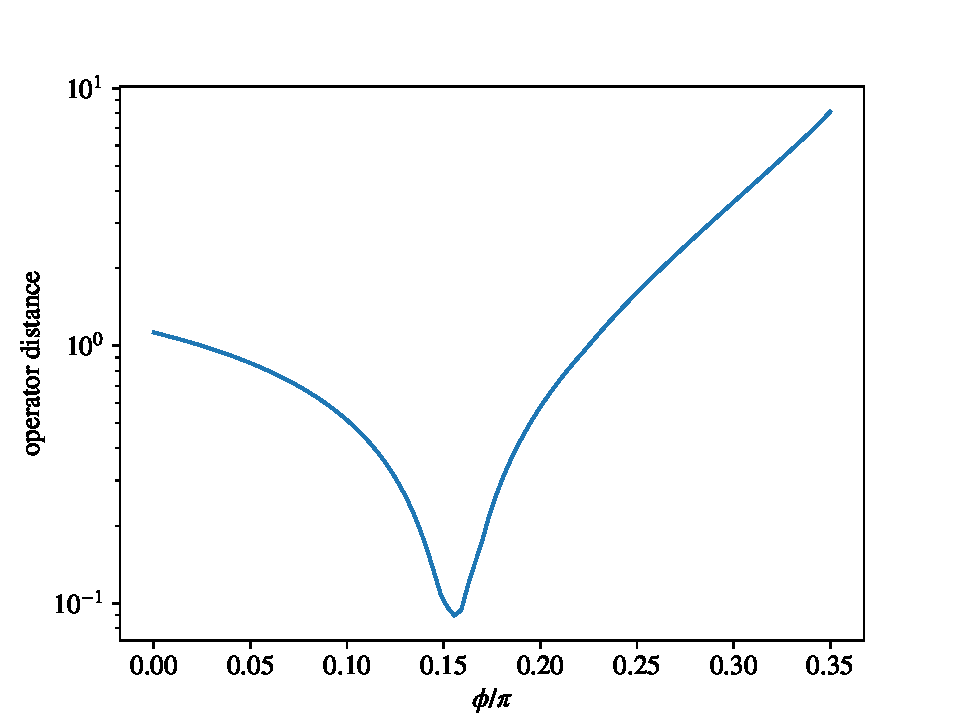
\includegraphics[height=0.15\textheight]{figure/zeta_distance_h1w6}
  (b)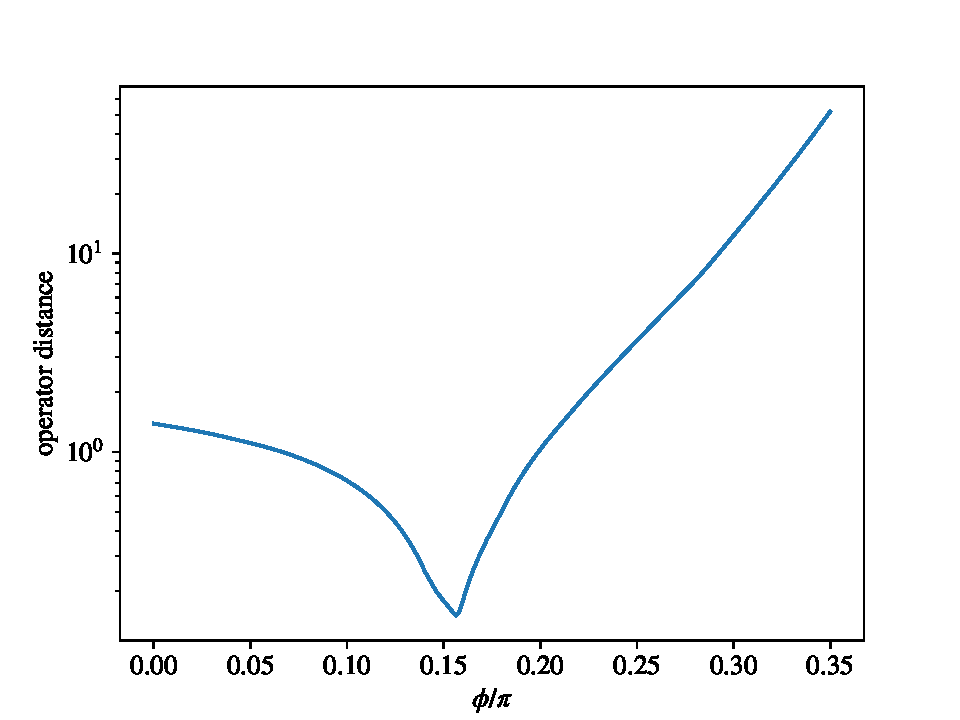
\includegraphics[height=0.15\textheight]{figure/zeta_distance_h1w10}
  (c)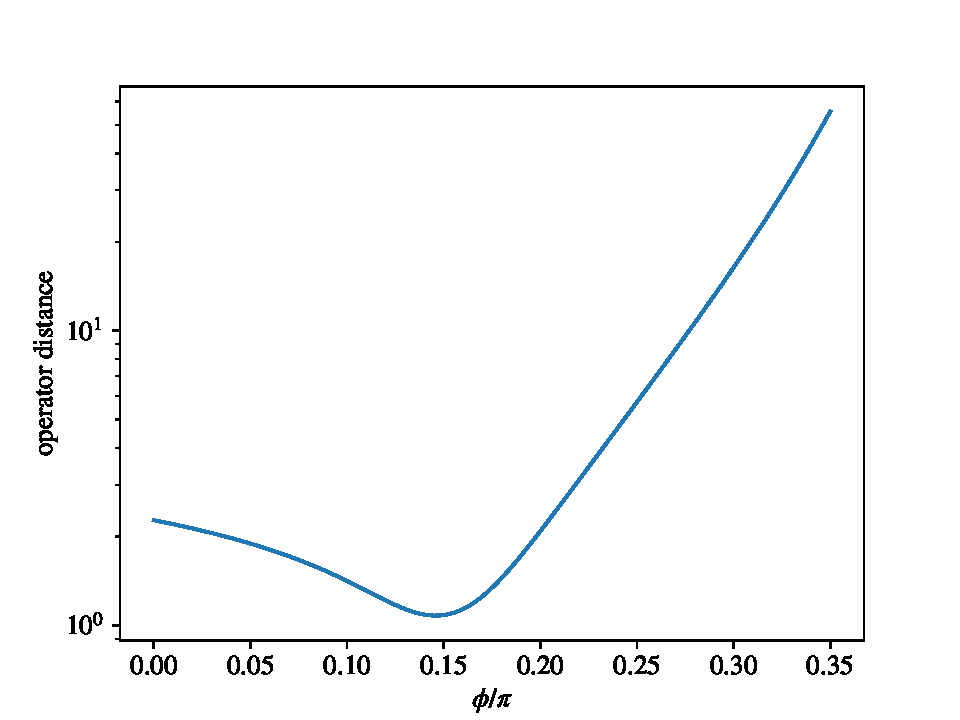
\includegraphics[height=0.15\textheight]{figure/zeta_distance_h3w3}
  \caption{The operator distance $\norm{\phi_A-\omega_A(\phi)}$ calculated in subsystems with size (a) $\mrm{height}=1$, $\mrm{width}=6$, (b) $\mrm{height}=1$, $\mrm{width}=10$, (c) $\mrm{height}=3$, $\mrm{width}=3$. The value of $\phi$ that makes the operator distance reaches the minima is about $\phi\approx 0.15\pi$, which is far from the value $\phi\approx 0.24\pi$ obtained by Ref.\cite{TN_Kitaev}.}\label{fig_TN_compare}
\end{figure}
Ref.\cite{TN_Kitaev} conjectured the following tensor-network state 
\[
\ket{\psi_{\mrm{SG}}(\phi)} = \mathcal{P}_A R_{\mrm{DG}}(\phi)\ket{(111)}
\]
gives a good approximation to the Kitaev spin liquid in the isotropic limit when the parameter $\phi$ is tuned to about $\phi\approx 0.24\pi$. The definition of the \emph{dimer-gas} operator $R_{\mrm{DG}}(\phi)$ is
\[
R_{\mrm{DG}}(\phi) \equiv \sum_{\mathcal{M}\in\Gamma_D}\lr{\tan\phi}^{\abs{\mathcal{M}}}\prod_{\anglelr{ij}\in\mathcal{M}}\lrg{ij}
\]
where $\Gamma_D$ is the set of all dimer configurations with no connected dimers. Such an operator together with the plaquette projector $\mathcal{P}_A$ is very similar to the structure of the density matrix constructed by our method. So I define a \emph{quasi}-density matrix $\omega_A$ as
\[
\omega_A(\phi) := \frac{1}{2^{N^A-N^A_p}}\mathcal{P}_A R_{\mrm{DG}}(\phi)
\]
satisfying $\Tr_A\omega_A=1$, and then see the \emph{distance} between this quasi-density matrix and the exact density matrix of the Kitaev model we have solved. I'm not sure if it is a density matrix because there's no proof shows it is positive definite or not. The operator distance I choose here is defined as 
\[\norm{\phi_A-\omega_A} := \Tr\sqrt{\lr{\rho_A - \omega_A}^2}\]
The dependence of the operator distance on the parameter $\phi$ is plotted in Fig.\ref{fig_TN_compare}. The results show the operator distance between $\rho_A$ and $\omega_A(\phi)$ tends to reach the minimum when $\phi\approx0.15\pi$, which is not even close to the value $\phi\approx0.24\pi$ obtained by Ref.\cite{TN_Kitaev}. Note that $\tan(0.15\pi)\approx0.51$ is very close to the nearest neighbor correlation function $\anglelr{ic_ic_j}\approx 0.52$. Although the sizes of the subsystems I chose are small, it doesn't seems the optimal value of $\phi$ tends to move toward $0.24\pi$ at all when I increase the size of the subsystem. So I guess the hypothesis that $\omega_A$ mimics the exact density matrix is possibly not correct. The trial wave function $\ket{(111)}$ could play an important role in such a string-gas Ansatze.


\subsection{Topological Entanglement Entropy}
 
\section{Discussions}
\alert{(Tensor Network)}

\appendix
\section{Sum Rule and Entropy Calculations}
Here I'd like to investigate if we can find some equations or identities about $\mathcal{C}_{\mathcal{M}}$ that make it possible for us to solve for such coefficients in the density matrix.

First of all, the most basic and useful property of a pure state $\rho$ is that it is a projector, which implies the property $\rho^2 = \rho$. According to eqn.(\ref{Crho.e}) with the projector condition, we have
\begin{align*}
  \rho^2 &= \mathcal{P}_G\lr{\frac{\mathds{1}+\tilde{W}_h}{2}} \lr{\frac{\mathds{1}+\tilde{W}_v}{2}}\prod_{p} \lr{\frac{\mathds{1}+W_p}{2}} \sum_{[\mathcal{M}],[\mathcal{M}']}\mathcal{C}_{\mathcal{M}}\mathcal{C}_{\mathcal{M}'} \lr{\prod_{\anglelr{ij}\in\mathcal{M}\oplus\mathcal{M}'} \lrg{ij}} \\
  &= \rho = \mathcal{P}_G\lr{\frac{\mathds{1}+\tilde{W}_h}{2}} \lr{\frac{\mathds{1}+\tilde{W}_v}{2}}\prod_{p} \lr{\frac{\mathds{1}+W_p}{2}} \sum_{[\mathcal{M}_b]}\mathcal{C}_{\mathcal{M}_b} \lr{\prod_{\anglelr{ij}\in\mathcal{M}_b} \lrg{ij}}
\end{align*}
where $\lrg{ij} \equiv \tilde{S}^{\alpha_{ij}}_i\tilde{S}^{\alpha_{ij}}_j$ After the comparison, we know that 
\[
\sum_{[\mathcal{M}],[\mathcal{M}']}\mathcal{C}_{\mathcal{M}}\mathcal{C}_{\mathcal{M}'} \lr{\prod_{\anglelr{ij}\in\mathcal{M}\oplus\mathcal{M}'} \lrg{ij}}
=
\sum_{[\mathcal{M}_b]}\mathcal{C}_{\mathcal{M}_b} \lr{\prod_{\anglelr{ij}\in\mathcal{M}_b} \lrg{ij}}
\]
More explicitly, 
\begin{equation}\label{pre-identity.e}
\mathop{\sum_{[\mathcal{M}],[\mathcal{M}']}}_{[\mathcal{M}\oplus\mathcal{M}'] = [\mathcal{M}_b]} \mathcal{C}_{\mathcal{M}}\mathcal{C}_{\mathcal{M}'} = \mathcal{C}_{\mathcal{M}_b}
\end{equation}

\alert{We shall be very careful that 
\[[\lrg{ij},\lrg{jk}]\neq 0\]
. Therefore, two dimer configurations $\mathcal{M}$ and $\mathcal{M}'$ sharing \textbf{an odd number of common endpoints} don't commute,
\[
\lr{\prod_{\anglelr{ij}\in\mathcal{M}}\lrg{ij}} \lr{\prod_{\anglelr{ij}\in\mathcal{M}'}\lrg{ij}} = -\lr{\prod_{\anglelr{ij}\in\mathcal{M}'}\lrg{ij}} \lr{\prod_{\anglelr{ij}\in\mathcal{M}}\lrg{ij}}
\]
thus it is not always true to write 
\[
\lr{\prod_{\anglelr{ij}\in\mathcal{M}}\lrg{ij}} \lr{\prod_{\anglelr{ij}\in\mathcal{M}'}\lrg{ij}} = \lr{\prod_{\anglelr{ij}\in\mathcal{M}\oplus\mathcal{M}'}\lrg{ij}}
\]
Instead, \textbf{\emph{the order of product is important}}. 

Nevertheless, we need to keep a fact in mind that \textbf{$\mathcal{C}_\mathcal{M}$ is non-zero only when the number of endpoints in $A$-sublattice of $\mathcal{M}$ is the same as the number of endpoints in $B$-sublattice.} If a configuration $\mathcal{M}_b$  doesn't obey the rule, then it can be shown that there are only two possibilities that either 
\begin{enumerate}
  \item [(i)]$\mathcal{M}_b$ can only be decomposed into two sub-configurations $\mathcal{M}_1$ and $\mathcal{M}_2$ in the way that $\mathcal{M}_b = \mathcal{M}_1\oplus\mathcal{M}_2$, where either $\mathcal{M}_1$ or $\mathcal{M}_2$ violates the rule, or
  \item [(ii)] Both $\mathcal{M}_1$ both $\mathcal{M}_2$ obey the rule but they share an odd number of common end points. 
  \item [(iii)] Similar to the previous situation but two configurations share an even number of end points.
\end{enumerate}
So in (\ref{pre-identity.e}), the combinations of configurations $\mathcal{M}$ and $\mathcal{M}'$ in the summation must be one of the above two situations. For the first situation, we know at least one of $\mathcal{C}_{\mathcal{M}}$ is zero so they contribute nothing. On the other hand, consider the second case, then the exchange of $\mathcal{M}$ and $\mathcal{M}'$ causes a sign flipping thus the two contributions cancel each other because of the relation $[\lrg{ij},\lrg{jk}]\neq 0$. \textbf{The only one thing that remains unknown is situation (iii)} since two configurations sharing an even number of end points commute so they can't cancel each other like cases with an odd number of common end points. 
}

\alert{
On the other hand, the situation of non-zero configurations obeying the rule that the number of type-$A$ end points is the same as the number of type-$B$ end points is simpler. There are only two cases for two configurations $\mathcal{M}$ and $\mathcal{M}'$ to combine to form a non-zero configuration $\mathcal{M}_b$ in the way that $\mathcal{M}\oplus\mathcal{M}' = \mathcal{M}_b$, either
\begin{enumerate}
  \item [(i)] both configurations $\mathcal{M}$ and $\mathcal{M}'$ are non-zero configurations, or
  \item [(ii)] one of $\mathcal{M}$ and $\mathcal{M}'$ is a zero configuration.
\end{enumerate}
To prove this fact, one can think how to add or remove some points into or out of a non-zero configuration $\mathcal{M}$ to form a new non-zero configuration $\mathcal{M}_b$, and the answer is clearly a set of points where the number of type-$A$ points is the same as the type-$B$ ones, so that the new configuration can still obeys the rule. 
}



So let's get back to the identity
\[
\mathop{\sum_{[\mathcal{M}],[\mathcal{M}']}}_{[\mathcal{M}\oplus\mathcal{M}'] = [\mathcal{M}_b]} \mathcal{C}_{\mathcal{M}}\mathcal{C}_{\mathcal{M}'} = \mathcal{C}_{\mathcal{M}_b}
\]
\alert{\textbf{Such an identity holds only when $\mathcal{M}_b$ is a non-zero configuration.}} In the summation, we only have to care about those pairs of classes such that $[\mathcal{M}\oplus\mathcal{M}'] = [\mathcal{M}_b]$, and 
\[[\mathcal{M}\oplus\mathcal{M}'] = [\mathcal{M}_b] = [\mathcal{M}\oplus(\mathcal{M}_b\oplus\mathcal{M})]\]
which implies $[\mathcal{M}'] = [\mathcal{M}_b\oplus\mathcal{M}]$ according to proposition.\ref{cancel.thm}. With this, the above identity for coefficients can be simplified as
\begin{equation}\label{CoeIdentity.e}
  \sum_{[\mathcal{M}]} \mathcal{C}_{\mathcal{M}} \mathcal{C}_{\mathcal{M}\oplus\mathcal{M}_b}
  =
  \mathcal{C}_{\mathcal{M}_b}
\end{equation}
Such a property implies the following chain rule,
\begin{equation}\label{ChainRule.e}
  \sum_{[\mathcal{M}_1]}\sum_{[\mathcal{M}_2]}\cdots \sum_{[\mathcal{M}_n]}\mathcal{C}_{\mathcal{M}_1} \mathcal{C}_{\mathcal{M}_1\oplus\mathcal{M}_2} \mathcal{C}_{\mathcal{M}_2\oplus\mathcal{M}_3}\cdots \mathcal{C}_{\mathcal{M}_{n-1}\oplus\mathcal{M}_{n}} = \mathcal{C}_{\mathcal{M}_n}
\end{equation}
\alert{(Matrix Structure?)} An interesting special case is when $\mathcal{M}_b=\varnothing$, which gives the identity
\begin{equation}\label{SquareIdentity.e}
  \sum_{[\mathcal{M}]}\mathcal{C}_{\mathcal{M}}^2 = \mathcal{C}_{\varnothing} = \frac{1}{2^{N_d}}
\end{equation}
\alert{(More...)}

\section{Dimer Configuration Algebra}
\begin{definition}
  A \emph{dimer configuration} $\mathcal{M}$ living on a lattice graph $\Lambda$ is a set of nearest bonds. The elements in $\mathcal{M}$ are denoted by $\anglelr{ij}$, which are called \emph{dimers}, standing for bonds connecting nearest end points $i$ and $j$. We denoted by $\mathfrak{M}$ the set of all dimer configurations.
\end{definition}
We are not going to give the rigorous mathematical definition of a graph here since one can find it in almost every book covering graph theory. 
\begin{definition}
  A point of the lattice is called a \emph{connected point} if it is connected by an even number, including zero, of dimers. Otherwise it is called a \emph{disconnected point}. A \emph{dimer string} in a dimer configuration $\mathcal{M}$ is a set of connected dimers with no points connected by more than two dimers. If we isolate these dimers that form a single dimer string from $\mathcal{M}$ to form a new configuration, which consists only one dimer string, then the two disconnected points in the new configuration are called \emph{end points} of such a dimer string.
\end{definition}
\begin{definition}
  $\oplus:\mathfrak{M}\times\mathfrak{M}\to\mathfrak{M}$ is a map defined by the following rule 
  \[\mathcal{M}_1\oplus\mathcal{M}_2 := \mathcal{M}_1\cup\mathcal{M}_2-\mathcal{M}_1\cap\mathcal{M}_2 = (\mathcal{M}_1-\mathcal{M}_2)\cup(\mathcal{M}_2-\mathcal{M}_1)\]
  if $\mathcal{M}_1,\mathcal{M}_2\in\mathfrak{M}$.
\end{definition}
we will see it is the $\mathbb{Z}_2$ nature of the spin operators gives this definition. Before that, we need to know some properties of $\oplus$.
\begin{theorem}
For any $\mathcal{M}_1,\mathcal{M}_2,\mathcal{M}_3\in\mathfrak{M}$, the following properties hold 
  \begin{itemize}
    \item $\mathcal{M}_1\oplus\varnothing = \mathcal{M}_1$
    \item $\mathcal{M}_1\oplus\mathcal{M}_1 = \varnothing$
    \item $\mathcal{M}_1\oplus\mathcal{M}_2 = \mathcal{M}_2\oplus\mathcal{M}_1$
    \item $(\mathcal{M}_1\oplus\mathcal{M}_2)\oplus\mathcal{M}_3 = \mathcal{M}_1\oplus(\mathcal{M}_2\oplus\mathcal{M}_3)$
  \end{itemize}
\end{theorem}

\alert{continue...}


\begin{theorem}\label{equ.thm}
  $[\mathcal{M}_1\oplus\mathcal{M}_2] = [\mathcal{\varnothing}]$ if and only if $[\mathcal{M}_1] = [\mathcal{M}_2]$.
\end{theorem}
\begin{proof}
  If $[\mathcal{M}_1\oplus\mathcal{M}_2] = [\mathcal{\varnothing}]$, then according to the definition of the equivalent class,
  \[
  \lr{\frac{\mathds{1}+\tilde{W}_h}{2}} \lr{\frac{\mathds{1}+\tilde{W}_v}{2}}\prod_{p} \lr{\frac{\mathds{1}+W_p}{2}} \prod_{\anglelr{ij}\in\mathcal{M}_1\oplus\mathcal{M}_2}\lrg{ij} = \lr{\frac{\mathds{1}+\tilde{W}_h}{2}} \lr{\frac{\mathds{1}+\tilde{W}_v}{2}}\prod_{p} \lr{\frac{\mathds{1}+W_p}{2}}
  \]
  \alert{(Here $\lrg{ij}$ are perfectly commutable $\mathbb{Z}_2$ operators living on dimers)} which, thanks to the fact that $\lrg{ij}$ are $\mathbb{Z}_2$ operators, immediately implies that
  \[
  \lr{\frac{\mathds{1}+\tilde{W}_h}{2}} \lr{\frac{\mathds{1}+\tilde{W}_v}{2}}\prod_{p} \lr{\frac{\mathds{1}+W_p}{2}} \prod_{\anglelr{ij}\in\mathcal{M}_1}\lrg{ij} = \lr{\frac{\mathds{1}+\tilde{W}_h}{2}} \lr{\frac{\mathds{1}+\tilde{W}_v}{2}}\prod_{p} \lr{\frac{\mathds{1}+W_p}{2}}
  \prod_{\anglelr{ij}\in\mathcal{M}_2}\lrg{ij}
  \]
  via multiplying the dimer configuration $\mathcal{M}_2$ to both side of the equation. Again, by the definition of the equivalent class, we conclude that $[\mathcal{M}_1] = [\mathcal{M}_2]$. The converse can be proved in the same way by multiplying the graph $\mathcal{M}_2$ back to get the original equation, and eventually the proof will be completed.
\end{proof}
\begin{theorem}\label{cancel.thm}
  For arbitrary $\mathcal{M},\mathcal{M}_1,\mathcal{M}_2\in\mathfrak{M}$, $[\mathcal{M}_1] = [\mathcal{M}_2]$ if and only if $[\mathcal{M}\oplus\mathcal{M}_1] = [\mathcal{M}\oplus\mathcal{M}_2]$
\end{theorem}
\begin{proof}
   It is obvious that $[\mathcal{M}_1] = [\mathcal{M}_2]$ implies $[\mathcal{M}_1\oplus\mathcal{M}] = [\mathcal{M}_2\oplus\mathcal{M}]$ for any $\mathcal{M}$, which can be proved by the method we used in thm.\ref{equ.thm}. Now, let $\mathcal{M}_1'=\mathcal{M}_1\oplus\mathcal{M}$ and $\mathcal{M}_2'=\mathcal{M}_2\oplus\mathcal{M}$, then we still know that $[\mathcal{M}_1']=[\mathcal{M}_2']$ implies $[\mathcal{M}_1'\oplus\mathcal{M}]=[\mathcal{M}_2'\oplus\mathcal{M}]$. Because 
  \[\mathcal{M}_1'\oplus\mathcal{M} = (\mathcal{M}_1\oplus\mathcal{M})\oplus\mathcal{M} = \mathcal{M}_1\oplus (\mathcal{M}\oplus\mathcal{M}) = \mathcal{M}_1\oplus \varnothing = \mathcal{M}_1\]
  and a similar result for $\mathcal{M}_2'$ obtained for the same reason, we then know that the converse statement of the proposition is also true. To this point the proof is completed.
\end{proof}

\begin{definition}
  The \emph{set of end points} of a dimer configuration $\mathcal{M}$ is a collection of end points of strings in the dimer configuration $\mathcal{M}$, which is denoted by $\mrm{Ed}(\mathcal{M})$.
\end{definition}

\begin{theorem}
  There exists a bijection from a equivalent class $[\mathcal{M}]$ to the set of end points $\mrm{Ed}(\mathcal{M})$. 
\end{theorem}
A simpler way to understand this statement is that $\mrm{Ed}(\mathcal{M}_1) = \mrm{Ed}(\mathcal{M}_2)$ \emph{if and only if} $[\mathcal{M}_1] = [\mathcal{M}_2]$. This theorem tells us that two dimer configurations are equivalent as long as they share the same end points, which can also be seen through observing Fig.\ref{PlaquetteEquivalent.f}.
\begin{definition}
  Given a sublattice $A$, we say $[\mathcal{M}]\subset A$ if $\mrm{Ed}(\mathcal{M})\subset A$
\end{definition}
We emphasize this definition because for an arbitrary $\mathcal{M}\in[\mathcal{M}_0]$, where $\mrm{Ed}(\mathcal{M}_0)\subset A$, it is not guaranteed that $\mathcal{M}\subset A$ because one can arbitrarily draw strings with parts outside the region $A$ as long as the end points are the same.



\section{Entanglement Entropy -- Perturbation}
Define a traceless matrix $\Sigma$ appears in the reduced density matrix,
\[
\rho_A = \frac{1}{2^{N^A}}\lr{\mathds{1} + \underbrace{\sum_{i\in A}\anglelr{\sigma_i^\mu} \sigma_i^\mu + \sum_{i>j\in A}\anglelr{\sigma^\mu_i\sigma^\nu_j}\sigma^\mu_i\sigma^\nu_j + \cdots}_{\equiv\Sigma}}  \equiv \frac{1}{2^{N^A}}\lr{\mathds{1} + \Sigma}
\]
Here we treat $\Sigma$ as a perturbation and calculate the entanglement entropy up to the second order of the correlation function.
\[
S_A = -\Tr_A\rho_A\ln\rho_A = N^A\ln 2 - \Tr_A \lrm{\rho_A\ln\lr{\mathds{1} + \Sigma}} \approx N^A\ln 2 - \Tr_A \lrm{\rho_A\lr{\Sigma - \frac{1}{2}\Sigma^2}} = N^A\ln 2 - \anglelr{\Sigma} + \frac{1}{2}\anglelr{\Sigma^2}
\]
The term $\anglelr{\Sigma}$ can be easily calculated,
\[
\anglelr{\Sigma} = \sum_{i\in A}\anglelr{\sigma_i^\mu}\anglelr{\sigma_i^\mu}  + \sum_{i>j\in A}\anglelr{\sigma^\mu_i\sigma^\nu_j}\anglelr{\sigma^\mu_i\sigma^\nu_j} + \cdots
\]
As for the second term $\anglelr{\Sigma^2}$,
\begin{align*}
  \anglelr{\Sigma^2} &= \anglelr{\lr{\sum_{i\in A}\anglelr{\sigma_i^\mu} \sigma_i^\mu + \sum_{i>j\in A}\anglelr{\sigma^\mu_i\sigma^\nu_j}\sigma^\mu_i\sigma^\nu_j + \cdots}^2} \\
  &= \sum_{ij\in A} \anglelr{ \sigma_i^\mu}\anglelr{\sigma_j^\nu}\anglelr{\sigma_i^\mu\sigma_j^\nu} + 2\sum_{k}\sum_{i>j\in A}\anglelr{\sigma^\mu_i\sigma^\nu_j}\anglelr{\sigma^\lambda_k} \anglelr{\sigma^\mu_i\sigma^\nu_j\sigma^\lambda_k} + \sum_{i>j\in A}\sum_{k>l\in A}\anglelr{\sigma^\mu_i\sigma^\nu_j}\anglelr{\sigma^\mu_k\sigma^\nu_l}\anglelr{\sigma^\mu_i\sigma^\nu_j\sigma^\mu_k\sigma^\nu_l } + \cdots \\
  &= \sum_{i\in A}\anglelr{\sigma_i^\mu}\anglelr{\sigma_i^\mu} + \sum_{i>j\in A} \lr{2\anglelr{\sigma_i^\mu}\anglelr{\sigma_j^\nu}\anglelr{\sigma_i^\mu\sigma_j^\nu} + \anglelr{\sigma^\mu_i\sigma^\nu_j}\anglelr{\sigma^\mu_i\sigma^\nu_j}}+\cdots 
\end{align*}
If the state preserves TRS, then those correlators containing odd numbers of spin operators vanish. Put them together, we obtain
\begin{equation}\label{TRS general enttropy.e}
  S_A \approx N^A\ln 2 - \frac{1}{2}\sum_{i>j\in A}\anglelr{\sigma^\mu_i\sigma^\nu_j}\anglelr{\sigma^\mu_i\sigma^\nu_j} + \cdots
\end{equation}

However, this perturbation scheme doesn't hold in the Kitaev model and toric code model because, for example, although the expectation value of a plaquette operator is a six-points correlation function,
\[
\anglelr{W_p} = \anglelr{\sigma^x_1\sigma^y_2\sigma^z_3\sigma^z_4\sigma^x_5\sigma^y_6} = 1
\]
it is nevertheless larger than any two-points correlation function $\anglelr{\sigma^\mu_i\sigma^\nu_j}$, so shouldn't be truncated as naively as we have done in the perturbation process to got (\ref{TRS general enttropy.e}).






\begin{thebibliography}{99}
    \bibitem{Qi}\href{https://doi.org/10.1103/PhysRevLett.105.080501}{H. Yao and X. L. Qi, \emph{Entanglement Entropy and Entanglement Spectrum of the Kitaev Model}, \emph{Phys. Rev. Lett.} \textbf{105}, 080501 (2010)}
    \bibitem{LevinTEE}\href{https://doi.org/10.1103/PhysRevLett.96.110405}{M. Levin, X. Wen, \emph{Detecting Topological Order in a Ground State Wave Function}, \emph{Phys. Rev. Lett.} \textbf{96}, 110405 (2006)}
    \bibitem{TNEE}\href{https://doi.org/10.1016/j.aop.2010.05.008}{N. Schuch, I. Cirac, D. P\'erez-Garc\'ia, \emph{PEPS as ground states: Degeneracy and topology}, \emph{Ann. Phys.} \textbf{325}, 2153 (2010)}
    \bibitem{majoaranacorrelation}\href{https://arxiv.org/abs/quant-ph/0304098}{J. I. Latorre, E. Rico, G. Vidal, \emph{Ground state entanglement in quantum spin chains},	arXiv:quant-ph/0304098}
    \bibitem{topoEE}\href{https://doi.org/10.1103/PhysRevLett.96.110404}{Alexei Kitaev and John Preskill, \emph{Topological Entanglement Entropy}, \emph{Phys. Rev. Lett.} 96, 110404 (2006)}
    \bibitem{Witten}\href{https://link.springer.com/article/10.1007/BF01217730}{E. Witten, \emph{Quantum field theory and the Jones polynomial}, \emph{Commun. Math. Phys.} \textbf{121}, 351 (1989)}
    \bibitem{TN_Kitaev}\href{https://doi.org/10.1103/PhysRevLett.123.087203}{Hyun-Yong Lee, Ryui Kaneko, Tsuyoshi Okubo, and Naoki Kawashima, \emph{Gapless Kitaev Spin Liquid to Classical String Gas through Tensor Networks}, \emph{Phys. Rev. Lett.} \textbf{123}, 087203 (2019)}
    \bibitem{ToricCodeTN}\href{https://doi.org/10.1103/PhysRevB.79.085118}{Zheng-Cheng Gu, Michael Levin, Brian Swingle, and Xiao-Gang Wen, \emph{Tensor-product representations for string-net condensed states}, \emph{Phys. Rev. B} \textbf{79}, 085118 (2009)}
    \bibitem{Baskaran}\href{https://doi.org/10.1103/PhysRevLett.98.247201}{G. Baskaran, Saptarshi Mandal, and R. Shankar, \emph{Exact Results for Spin Dynamics and Fractionalization in the Kitaev Model}, \emph{Phys. Rev. Lett.} \textbf{98}, 247201 (2007)}
    \bibitem{BCref1}\href{https://doi.org/10.1103/PhysRevB.75.134415}{Wojciech Brzezicki, Jacek Dziarmaga, Andrzej M. Ole\'s, \emph{Quantum phase transition in the one-dimensional compass model}, \emph{Phys. Rev. B} \textbf{75}, 134415 (2007)}
    \bibitem{BCref2}\href{https://doi.org/10.1103/PhysRevB.80.174417}{Ke-Wei Sun and Qing-Hu Chen, \emph{Quantum phase transition of the one-dimensional transverse-field compass model}, \emph{Phys. Rev. B} \textbf{80}, 174417 (2009)}
    \bibitem{Peschel}\href{https://doi.org/10.1088/0305-4470/36/14/101}{Ingo Peschel, \emph{Calculation of reduced density matrices from correlation functions}, \emph{J. Phys. A: Math. Gen.} \textbf{36}, L205 (2003)}
\end{thebibliography}
\end{document} 